%% LeJEPA Presentation Slides
%% Template: WASA-style (Metropolis) × LeJEPA color scheme
%% Compile: xelatex lejepa_slides.tex (twice)

\documentclass[aspectratio=169,9pt]{beamer}

\usetheme{metropolis}
\usepackage[utf8]{inputenc}
\usepackage[T5]{fontenc}
\usepackage{amsmath,amssymb,bm}
\usepackage{booktabs}
\usepackage{tikz}
\usepackage{tikz-3dplot}
\usetikzlibrary{
  arrows.meta, positioning, shapes.geometric, fit, backgrounds,
  calc, decorations.pathreplacing, decorations.markings, patterns, 3d
}
\usepackage{pgfplots}
\pgfplotsset{compat=1.18}
\usepackage{xcolor}
\usepackage{graphicx}
\usepackage{mathtools}
\usepackage{mdframed}
\usepackage{array}
\usepackage{pifont}
\usepackage{listings}
\usepackage[numbers,compress]{natbib}
\renewcommand{\bibfont}{\tiny}
\newcommand{\cmark}{\ding{51}}
\newcommand{\xmark}{\ding{55}}

%% ─── Color Palette: WASA-style + LeJEPA Navy/Gold ───────────────────────────
\definecolor{mprimary}{HTML}{2C3E6B}   % Navy (LeJEPA primary)
\definecolor{maccent}{HTML}{C8A951}    % Gold
\definecolor{mgood}{HTML}{5B8C6B}      % Sage green
\definecolor{mbad}{HTML}{B85450}       % Terracotta
\definecolor{mgray}{HTML}{9E9E9E}      % Mid gray
\definecolor{mdark}{HTML}{212121}      % Near-black (header)
\definecolor{mlight}{HTML}{EEF0F5}     % Light blue-gray
\definecolor{mlightgold}{HTML}{F5F0E0} % Light gold
\definecolor{mlightsage}{HTML}{E5EDE8} % Light sage
\definecolor{mlightred}{HTML}{F2E6E5}  % Light terracotta

\setbeamercolor{frametitle}{bg=mdark, fg=white}
\setbeamercolor{progress bar}{fg=mprimary}
\setbeamercolor{structure}{fg=mprimary}
\setbeamercolor{title separator}{fg=maccent}

%% ─── mdframed Box Styles ─────────────────────────────────────────────────────
\newmdenv[
  topline=false, bottomline=false, rightline=false,
  linewidth=3pt, linecolor=mprimary!60,
  innerleftmargin=10pt, innerrightmargin=6pt,
  innertopmargin=5pt, innerbottommargin=5pt,
  backgroundcolor=mlight
]{primarybox}

\newmdenv[
  topline=false, bottomline=false, rightline=false,
  linewidth=3pt, linecolor=mgood!70,
  innerleftmargin=10pt, innerrightmargin=6pt,
  innertopmargin=5pt, innerbottommargin=5pt,
  backgroundcolor=mlightsage
]{goodbox}

\newmdenv[
  topline=false, bottomline=false, rightline=false,
  linewidth=3pt, linecolor=mbad!70,
  innerleftmargin=10pt, innerrightmargin=6pt,
  innertopmargin=5pt, innerbottommargin=5pt,
  backgroundcolor=mlightred
]{badbox}

\newmdenv[
  topline=false, bottomline=false, rightline=false,
  linewidth=3pt, linecolor=maccent!80,
  innerleftmargin=10pt, innerrightmargin=6pt,
  innertopmargin=5pt, innerbottommargin=5pt,
  backgroundcolor=mlightgold
]{accentbox}

%% ─── Takeaway Banner ─────────────────────────────────────────────────────────
\newcommand{\takeaway}[1]{%
  \vfill
  \begin{mdframed}[
    linecolor=maccent, linewidth=1.5pt,
    backgroundcolor=mlightgold,
    innertopmargin=5pt, innerbottommargin=5pt,
    innerleftmargin=10pt, innerrightmargin=10pt,
    roundcorner=3pt, skipabove=4pt, skipbelow=0pt
  ]
  \centering\small\bfseries\color{mprimary} #1
  \end{mdframed}%
}

%% ─── TikZ styles ─────────────────────────────────────────────────────────────
\tikzset{
  pbox/.style={draw=mprimary!50, fill=mlight, rounded corners=3pt,
               minimum height=0.65cm, font=\small, inner sep=5pt},
  gbox/.style={draw=mgood!60, fill=mlightsage, rounded corners=3pt,
               minimum height=0.65cm, font=\small, inner sep=5pt},
  rbox/.style={draw=mbad!60, fill=mlightred, rounded corners=3pt,
               minimum height=0.65cm, font=\small, inner sep=5pt},
  abox/.style={draw=maccent!70, fill=mlightgold, rounded corners=3pt,
               minimum height=0.65cm, font=\small, inner sep=5pt},
  darkbox/.style={draw=mprimary, fill=mprimary!85, text=white, rounded corners=3pt,
                  minimum height=0.7cm, font=\small\bfseries, inner sep=6pt},
  arr/.style={->, thick, mprimary},
  darr/.style={->, dashed, thin, mgray},
}

%% ─── Title ───────────────────────────────────────────────────────────────────
\title{\textbf{LeJEPA}\\
       \large Provable \& Scalable Self-Supervised Learning}
\subtitle{Without the Heuristics \quad\textcolor{mgray}{\small Balestriero \& LeCun, arXiv:2511.08544}}
\author{}
\date{}

% ═══════════════════════════════════════════════════════════════════════════════
\begin{document}
% ═══════════════════════════════════════════════════════════════════════════════

% ─── Title Slide (custom) ─────────────────────────────────────────────────────
\begin{frame}[plain]
\vspace{0.4cm}
\begin{columns}[c]
\column{0.48\textwidth}
  \begin{center}
    {\Huge\bfseries\color{mprimary} LeJEPA}\\[6pt]
    {\large\itshape\color{mprimary!80} Provable \& Scalable SSL}\\[4pt]
    {\normalsize\itshape Without the Heuristics}\\[14pt]
    {\small\color{mgray} Randall Balestriero \& Yann LeCun (2025)}\\[3pt]
    {\small\color{mgray} arXiv:~2511.08544}\\[12pt]
    {\small\bfseries\color{mprimary} Presenter: Continuer team}
  \end{center}

\column{0.50\textwidth}
\begin{center}
\begin{tikzpicture}[every node/.style={font=\small}, scale=0.95]

  %% Input — fan-stacked photos (back to front)
  \begin{scope}[yshift=0.12cm]
    % Back photo: navy, tilted -14°
    \begin{scope}[rotate around={-14:(-0.12,0)}]
      \fill[mprimary!11, rounded corners=3pt] (-0.59,-0.62) rectangle (0.35,0.62);
      \fill[mprimary!23]                      (-0.59, 0.08) rectangle (0.35,0.62);
      \fill[mprimary!38, opacity=0.72]        (-0.12,-0.16) ellipse (0.17 and 0.21);
      \draw[mprimary!32, line width=0.6pt, rounded corners=3pt] (-0.59,-0.62) rectangle (0.35,0.62);
    \end{scope}

    % Middle photo: sage, tilted +7°
    \begin{scope}[rotate around={7:(0.10,-0.05)}]
      \fill[mgood!10, rounded corners=3pt] (-0.37,-0.67) rectangle (0.57,0.57);
      \fill[mgood!20]                      (-0.37, 0.05) rectangle (0.57,0.57);
      \fill[mgood!38, opacity=0.72]        (0.10,-0.18) ellipse (0.17 and 0.21);
      \draw[mgood!33, line width=0.6pt, rounded corners=3pt] (-0.37,-0.67) rectangle (0.57,0.57);
    \end{scope}

    % Front photo: warm gold, straight
    \fill[maccent!11, rounded corners=3pt] (-0.19,-0.72) rectangle (0.75,0.48);
    \fill[maccent!23]                      (-0.19,-0.04) rectangle (0.75,0.48);
    \fill[maccent!42, opacity=0.72]        (0.28,-0.24) ellipse (0.17 and 0.21);
    \draw[maccent!38, line width=0.6pt, rounded corners=3pt] (-0.19,-0.72) rectangle (0.75,0.48);

    % Invisible anchor for label
    \node[inner sep=0, minimum width=2.0cm, minimum height=1.5cm] (img) at (0.08,-0.10) {};
    \node[font=\tiny, mgray, below=6pt of img] {Dữ liệu};
  \end{scope}

  %% Encoder box
  \node[darkbox, minimum width=1.1cm, minimum height=0.75cm] (enc) at (2.2,0) {$f_\theta$};
  \node[font=\tiny, mgray, below=3pt of enc] {Bộ mã hóa};

  %% Arrow: right edge of front photo → enc
  \draw[->, thick, mprimary] (0.77, 0) -- (enc.west);

  %% Embedding dots
  \fill[mgood!80] (4.0,  0.0) circle (4.5pt);
  \fill[mgood!80] (4.45, 0.7) circle (3.8pt);
  \fill[mgood!80] (4.5, -0.6) circle (4.2pt);
  \fill[mgood!80] (5.05, 0.3) circle (3.4pt);
  \fill[mgood!80] (4.95,-1.0) circle (3.8pt);

  %% Dashed Gaussian circle
  \draw[dashed, mgood!60, line width=1.1pt] (4.55, -0.18) circle (1.38cm);
  \node[font=\scriptsize, mgood] at (5.85, 1.05) {$\mathcal{N}(0,I)$};

  %% Arrows enc -> embeddings
  \foreach \x/\y in {4.0/0.0, 4.45/0.7, 4.5/-0.6, 5.05/0.3, 4.95/-1.0}{
    \draw[->, thick, mgood!70] (enc.east) -- (\x,\y);
  }

\end{tikzpicture}
\end{center}
\end{columns}
\end{frame}

\begin{frame}{Nội Dung Trình Bày}
\vspace{0.8cm}
\begin{center}
\begin{tikzpicture}[x=3.5cm, y=1cm]
  \tikzstyle{stepbox} = [draw=mprimary!40, fill=white, rounded corners=6pt, text width=2.6cm, align=center, inner sep=6pt, minimum height=1.6cm, line width=1.2pt]
  \tikzstyle{stepnum} = [circle, fill=mprimary, text=white, font=\large\bfseries, inner sep=0pt, minimum size=0.8cm]
  
  %% Connecting Line
  \draw[line width=2pt, mprimary!20] (0, 1.5) -- (3, 1.5);

  %% Step 1
  \node[stepbox, draw=mprimary] (b1) at (0, -0.2) {\textbf{\color{mprimary}WHAT}\\[3pt]\scriptsize Học biểu diễn là gì?};
  \node[stepnum, fill=mprimary] (n1) at (0, 1.5) {1};
  \draw[thick, mprimary] (n1) -- (b1);

  %% Step 2
  \node[stepbox, draw=mbad] (b2) at (1, -0.2) {\textbf{\color{mbad}WHY}\\[3pt]\scriptsize Tại sao JEPA thất bại?};
  \node[stepnum, fill=mbad] (n2) at (1, 1.5) {2};
  \draw[thick, mbad] (n2) -- (b2);

  %% Step 3
  \node[stepbox, draw=mgood] (b3) at (2, -0.2) {\textbf{\color{mgood}HOW}\\[3pt]\scriptsize Giải quyết từ gốc rễ};
  \node[stepnum, fill=mgood] (n3) at (2, 1.5) {3};
  \draw[thick, mgood] (n3) -- (b3);

  %% Step 4
  \node[stepbox, draw=maccent] (b4) at (3, -0.2) {\textbf{\color{maccent}RESULTS}\\[3pt]\scriptsize Đánh giá thực nghiệm};
  \node[stepnum, fill=maccent] (n4) at (3, 1.5) {4};
  \draw[thick, maccent] (n4) -- (b4);

\end{tikzpicture}
\end{center}

\vspace{0.5cm}
\begin{accentbox}
\centering\small
\textit{“LeJEPA: Tối giản hóa self-supervised learning bằng nền tảng lý thuyết vững chắc.”}
\end{accentbox}
\end{frame}

% ─── Slide: Short Glossary ───────────────────────────────────────────────────
\begin{frame}{Thuật Ngữ Trọng Tâm}
  \vspace{0.3em}
  Các khái niệm cốt lõi thường xuyên xuất hiện trong bài trình bày:
  
  \vspace{0.6em}
  \begin{enumerate}\small\setlength\itemsep{1em}
    \item \textbf{\color{mprimary}Anisotropic / Isotropic:} Bất đẳng hướng (các hướng không đều) / Đẳng hướng (phân bố đều mọi hướng).
    \item \textbf{\color{mprimary}SSL:} Self-Supervised Learning (Học máy tự giám sát).
    \item \textbf{\color{mprimary}Random projection:} Phép chiếu ngẫu nhiên (chuyển không gian dữ liệu nhiều chiều xuống ít chiều hơn).
    \item \textbf{\color{mprimary}Decision boundary:} Ranh giới quyết định (đường/mặt phân tách các nhóm dữ liệu trong mô hình).
    \item \textbf{\color{mprimary}Exploding gradients:} Bùng nổ đạo hàm (đạo hàm tăng quá lớn khiến mô hình không thể huấn luyện).
  \end{enumerate}
\end{frame}


% ─── SECTION DIVIDER ──────────────────────────────────────────────────────────
\section{WHAT — Học biểu diễn là gì?}

% ─── Slide 1: Foundation model goal ──────────────────────────────────────────
\begin{frame}{Mục Tiêu: Encoder Ánh Xạ Thế Giới Vào Không Gian Có Ý Nghĩa}

\begin{columns}[T]
\column{0.50\textwidth}

Học $f_\theta : \mathbb{R}^D \to \mathbb{R}^K$ sao cho embedding \textbf{có ích cho mọi downstream task} — không cần nhãn trong lúc huấn luyện.

\vspace{0.7em}
\begin{tikzpicture}[scale=0.88, every node/.style={font=\small}]
  %% Input
  \node[pbox, minimum width=1.0cm] (x) at (0,0) {$\mathbf{x}$};
  \node[font=\tiny, mgray, below=2pt of x] {ảnh / video / text};

  %% Encoder
  \node[darkbox, minimum width=1.3cm, minimum height=1.0cm] (enc) at (2.3,0) {$f_\theta$};

  %% Latent space — ink-blot shape
  \begin{scope}[xshift=4.2cm, yshift=0cm]
    \node[font=\tiny, mgray] at (0.8, 1.15) {$\mathbb{R}^K$};
    % Blob
    \draw[mprimary!25, fill=mprimary!7, thick, line width=1pt]
      plot[smooth cycle, tension=0.75] coordinates {
        (0.1,0.3) (0.2,0.9) (0.6,1.0) (1.1,0.85)
        (1.6,0.65) (1.7,0.1) (1.2,-0.35) (0.6,-0.4) (0.0,-0.1)
      };
    % Clusters of dots
    \foreach \x/\y/\c in {
      0.35/0.55/mgood, 0.55/0.75/mgood, 0.4/0.85/mgood,
      1.0/0.65/mprimary, 1.2/0.5/mprimary, 1.1/0.3/mprimary,
      0.75/0.0/maccent, 0.6/-0.2/maccent}{
      \fill[\c, opacity=0.85] (\x,\y) circle (2.2pt);
    }
    % Cluster labels
    \node[font=\tiny, mgood]   at (0.35,0.35) {cat};
    \node[font=\tiny, mprimary] at (1.3,0.7)  {dog};
    \node[font=\tiny, maccent]  at (0.55,-0.35){sky};
  \end{scope}

  \draw[arr] (x) -- (enc);
  \draw[arr] (enc) -- (4.0, 0);
\end{tikzpicture}

\column{0.47\textwidth}
\vspace{0.4em}

Một $f_\theta$ tốt phục vụ được nhiều task:

\vspace{0.4em}
\begin{tikzpicture}[every node/.style={font=\footnotesize}, scale=0.88]
  \node[pbox, minimum width=0.7cm] (z) at (0,0) {$\mathbf{z}$};
  \foreach \ang/\lbl/\col in {
    70/Phân loại/mgood,
    10/Segmentation/mprimary,
    -45/Few-shot/maccent,
    -100/Retrieval/mgray}{
    \node[\col!90, align=left] (t) at (\ang:2.4cm) {\lbl};
    \draw[->, thin, \col!60] (z) -- (t);
  }
\end{tikzpicture}

\end{columns}

\vspace{0.3em}
\begin{primarybox}
\footnotesize \textbf{Foundation model:} một hệ thống giải được nhiều downstream task sau khi huấn luyện một lần, không thay đổi tham số $\theta$.
\end{primarybox}

\end{frame}


% ─── Slide 2: JEPA mechanism ─────────────────────────────────────────────────
\begin{frame}{JEPA: Dự Đoán Trạng Thái Trừu Tượng — Không Phải Pixel}

\begin{columns}[T]
\column{0.56\textwidth}

\vspace{0.3em}
\begin{tikzpicture}[every node/.style={font=\tiny}, scale=0.82, transform shape]
  % Ảnh gốc
  \node[pbox, minimum width=0.9cm, minimum height=0.55cm] (src) at (0.0, 0.0) {$x$};
  \node[font=\tiny, below=3pt of src] {Ảnh gốc};
  % Views
  \node[pbox, minimum width=0.9cm, minimum height=0.55cm] (v1) at (1.4,  0.7) {view 1};
  \node[pbox, minimum width=0.9cm, minimum height=0.55cm] (v2) at (1.4, -0.7) {view 2};
  \draw[darr] (src.north east) -- (v1.west);
  \draw[darr] (src.south east) -- (v2.west);
  % Encoders
  \node[darkbox, minimum width=0.9cm, minimum height=0.55cm] (e1) at (2.8,  0.7) {$f_\theta$};
  \node[darkbox, minimum width=0.9cm, minimum height=0.55cm] (e2) at (2.8, -0.7) {$f_\theta$};
  \draw[arr] (v1) -- (e1);
  \draw[arr] (v2) -- (e2);
  % Latents
  \node[abox, minimum width=0.7cm, minimum height=0.55cm] (z1) at (4.0,  0.7) {$z_1$};
  \node[abox, minimum width=0.7cm, minimum height=0.55cm] (z2) at (4.0, -0.7) {$z_2$};
  \draw[arr] (e1) -- (z1);
  \draw[arr] (e2) -- (z2);
  % Predictor + ẑ_1
  \node[darkbox, minimum width=1.1cm, minimum height=0.55cm] (pred) at (5.4, -0.7) {Dự báo};
  \node[abox,  minimum width=0.7cm, minimum height=0.55cm] (zh)   at (6.8, -0.7) {$\hat{z}_1$};
  \draw[arr] (z2)   -- (pred);
  \draw[arr] (pred) -- (zh);
  % Loss
  \node[gbox, draw=mgood!80, text=mprimary, font=\small\bfseries,
        minimum width=1.1cm, minimum height=0.65cm] (loss) at (8.2, -0.7) {Loss};
  \draw[arr] (zh) -- (loss);
  % z1 → loss: đi ngang hàng trên rồi thả xuống
  \draw[arr] (z1.east) -- (8.2, 0.7) -- (loss.north);
  % Shared encoder background
  \begin{pgfonlayer}{background}
    \node[draw=mgray, dashed, fill=mgray!5, rounded corners=4pt,
          fit=(e1)(e2), inner sep=5pt] (encbox) {};
  \end{pgfonlayer}
  \node[font=\tiny, color=mgray, above=3pt of encbox] {chia sẻ trọng số};
\end{tikzpicture}

\column{0.41\textwidth}
\vspace{0.5em}

\textbf{View} có thể là: crop, mask, blur, frame liền kề, modal khác…

\vspace{0.6em}
\begin{goodbox}
\footnotesize \textbf{JEPA} $\neq$ reconstruction: không khôi phục pixel mà học ``thế giới thay đổi thế nào'' ở mức trừu tượng.
\end{goodbox}

\vspace{0.6em}
Tuy nhiên, bài toán dự đoán có một \textbf{nghiệm tầm thường nguy hiểm}…

\end{columns}

\takeaway{JEPA: học trạng thái latent — không học pixel}

\end{frame}


% ─── SECTION DIVIDER ──────────────────────────────────────────────────────────
\section{WHY — Tại sao JEPA thất bại?}


% ─── Slide 3: Collapse explained ─────────────────────────────────────────────
\begin{frame}{Collapse — Khi Encoder Học Cách "Gian Lận"}

Việc cực tiểu hóa loss prediction $\|z_1 - \hat z_1\|^2$ có nghiệm hiển nhiên: \textbf{Collapse}. Mọi input đều bị ánh xạ về một cấu trúc vô dụng, loss giảm về 0 nhưng encoder không học được gì.

\vspace{0.4cm}
\begin{center}
\begin{tikzpicture}[every node/.style={font=\small}, scale=0.9]

  %% Subfig 1: Complete Collapse
  \node[mbad, font=\small\bfseries] at (0, 2.5) {Complete Collapse};
  % Input dots converging to one point
  \foreach \x/\y in {-1.5/1.2, -0.8/1.6, 0/1.4, 0.8/1.6, 1.5/1.2, -0.4/0.9, 0.4/0.9}{
    \fill[mbad!50] (\x,\y) circle (2.5pt);
    \draw[->, very thin, mbad!40] (\x,\y-0.15) -- (0, 0.15);
  }
  % Collapsed point
  \fill[mbad] (0,0) circle (6pt);
  \node[mbad, font=\scriptsize\bfseries, below=4pt] at (0,0) {$f_\theta(\mathbf{x}) = c \;\; \forall \mathbf{x}$};

  %% Separator
  \draw[dashed, mgray!40] (3.5, -0.5) -- (3.5, 2.8);

  %% Subfig 2: Dimensional Collapse
  \node[maccent, font=\small\bfseries] at (7, 2.5) {Dimensional Collapse};
  % A flat 1D line in 2D space
  \draw[thick, maccent!40] (4.5, 0.5) -- (9.5, 0.5);
  % Dots mapped onto the line only
  \foreach \x in {4.8, 5.5, 6.1, 7.0, 7.8, 8.5, 9.2}{
    \fill[maccent] (\x,0.5) circle (3.5pt);
  }
  \node[maccent, font=\scriptsize\bfseries, below=4pt] at (7,0.5) {Sống trên không gian con chiều thấp};

\end{tikzpicture}
\end{center}

\vspace{0.2cm}
\begin{columns}[T]
\column{0.48\textwidth}
\begin{badbox}
\footnotesize \textbf{Complete collapse:}\\ Mất toàn bộ thông tin về input.
\end{badbox}

\column{0.48\textwidth}
\begin{accentbox}
\footnotesize \textbf{Dimensional collapse:}\\ Representation kém đa dạng, downstream task hỏng.
\end{accentbox}
\end{columns}

\vspace{0.5cm}
\begin{center}
\footnotesize \textbf{Vấn đề:} Không có lý thuyết nào chỉ ra \emph{chính xác} phải làm gì để tránh collapse \textbf{mà vẫn tối ưu} cho downstream task.
\end{center}

\end{frame}


% ─── Slide 4: Literature timeline ────────────────────────────────────────────
\begin{frame}{Literature: Mỗi Phương Pháp Vá Một Lỗ Hổng Mới}

\vfill
\begin{center}
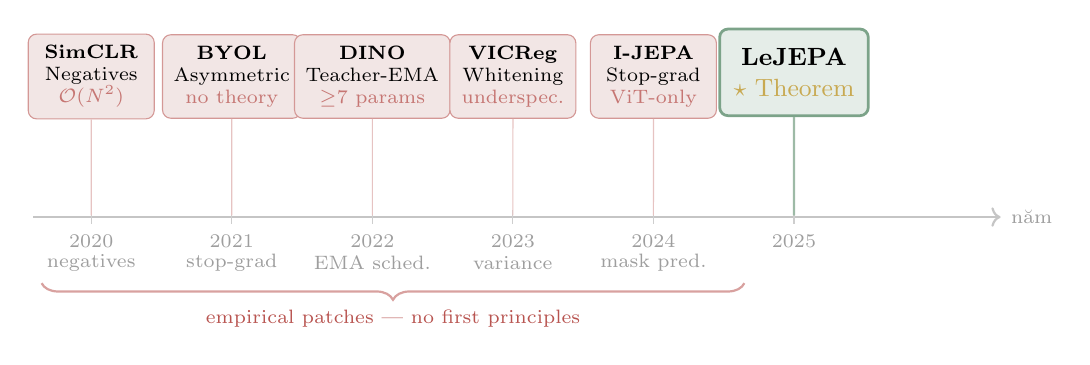
\begin{tikzpicture}[scale=1.05, every node/.style={font=\small}]
  %% Timeline axis
  \draw[->, thick, mgray!60] (-0.2,0) -- (11.5,0)
    node[right, mgray, font=\scriptsize]{năm};
  \foreach \x/\yr in {0.5/2020, 2.2/2021, 3.9/2022, 5.6/2023, 7.3/2024, 9.0/2025}{
    \draw[mgray!50] (\x,0.08) -- (\x,-0.08);
    \node[mgray, font=\scriptsize, below=3pt] at (\x,0) {\yr};
  }

  %% Heuristic method boxes — slightly taller for readability
  \node[rbox, minimum width=1.6cm, minimum height=1.0cm, align=center, font=\scriptsize, inner sep=4pt]
    (mA) at (0.5,1.7) {\textbf{SimCLR}\\Negatives\\\textcolor{mbad!80}{$\mathcal{O}(N^2)$}};
  \draw[mbad!35,thin] (mA.south)--(0.5,0.02);

  \node[rbox, minimum width=1.6cm, minimum height=1.0cm, align=center, font=\scriptsize, inner sep=4pt]
    (mB) at (2.2,1.7) {\textbf{BYOL}\\Asymmetric\\\textcolor{mbad!80}{no theory}};
  \draw[mbad!35,thin] (mB.south)--(2.2,0.02);

  \node[rbox, minimum width=1.6cm, minimum height=1.0cm, align=center, font=\scriptsize, inner sep=4pt]
    (mC) at (3.9,1.7) {\textbf{DINO}\\Teacher-EMA\\\textcolor{mbad!80}{$\geq$7 params}};
  \draw[mbad!35,thin] (mC.south)--(3.9,0.02);

  \node[rbox, minimum width=1.6cm, minimum height=1.0cm, align=center, font=\scriptsize, inner sep=4pt]
    (mD) at (5.6,1.7) {\textbf{VICReg}\\Whitening\\\textcolor{mbad!80}{underspec.}};
  \draw[mbad!35,thin] (mD.south)--(5.6,0.02);

  \node[rbox, minimum width=1.6cm, minimum height=1.0cm, align=center, font=\scriptsize, inner sep=4pt]
    (mE) at (7.3,1.7) {\textbf{I-JEPA}\\Stop-grad\\\textcolor{mbad!80}{ViT-only}};
  \draw[mbad!35,thin] (mE.south)--(7.3,0.02);

  %% LeJEPA — highlight, taller
  \node[gbox, minimum width=1.75cm, minimum height=1.1cm, align=center,
        draw=mgood!80, line width=1pt, font=\small, inner sep=5pt]
    (lj) at (9.0, 1.75)
    {\textbf{LeJEPA}\\\textcolor{maccent}{$\star$ Theorem}};
  \draw[mgood!60, thick] (lj.south) -- (9.0, 0.02);

  %% Patch labels below axis
  \foreach \x/\lbl in {
    0.5/negatives, 2.2/stop-grad, 3.9/EMA sched., 5.6/variance, 7.3/mask pred.}{
    \node[mgray, font=\scriptsize] at (\x, -0.55) {\lbl};
  }

  %% Brace
  \draw[decorate, decoration={brace, mirror, amplitude=6pt}, mbad!55, thick]
    (-0.1,-0.8) -- (8.4,-0.8)
    node[midway, below=6pt, font=\scriptsize, mbad]
      {empirical patches — no first principles};

\end{tikzpicture}
\end{center}
\vfill
\takeaway{Câu hỏi sai: \emph{``tránh collapse thế nào?''} $\;\longrightarrow\;$ Câu hỏi đúng: \emph{``phân phối nào là tối ưu?''}}

\end{frame}


% ─── SECTION DIVIDER ──────────────────────────────────────────────────────────
\section{HOW — Giải từ gốc rễ}


% ─── Slide 5: The right question ─────────────────────────────────────────────
\begin{frame}{Phân phối Nào Là Tối Ưu Cho Foundation Model?}

\begin{columns}[T]
\column{0.50\textwidth}

Xét downstream task qua linear probe (ridge regression):
\[
  \hat\beta = \arg\min_\beta \|\mathbf{y} - \mathbf{Z}\beta\|^2 + \lambda\|\beta\|^2
\]

\vspace{0.4em}
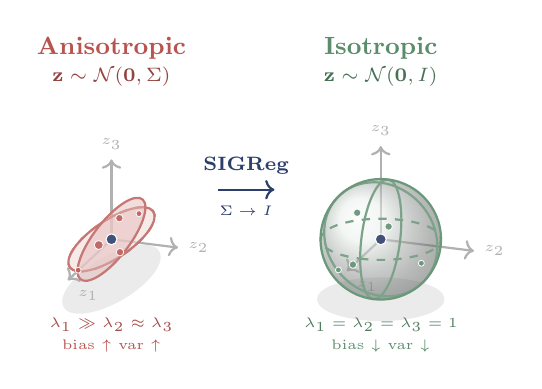
\begin{tikzpicture}[scale=0.9, every node/.style={font=\small}, line join=round]
  \tdplotsetmaincoords{70}{110}
  
  %% ── Anisotropic (left) ──
  \begin{scope}[xshift=1.0cm]
    \node[mbad, font=\small\bfseries] at (0, 2.5) {Anisotropic};
    \node[font=\scriptsize, mbad!80!black] at (0, 2.1) {$\mathbf{z} \sim \mathcal{N}(\mathbf{0}, \Sigma)$};
    
    \begin{scope}[yshift=-0.2cm]
      \begin{scope}[tdplot_main_coords]
        % Shadow
        \begin{scope}[canvas is xy plane at z=-0.6]
          \fill[mgray!30, opacity=0.7] (0,0) ellipse (1.5cm and 0.5cm);
        \end{scope}
        
        % 3D Axes
        \draw[->, thick, mgray!80] (0,0,0) -- (1.8,0,0) node[anchor=north west, font=\tiny]{$z_1$};
        \draw[->, thick, mgray!80] (0,0,0) -- (0,1.0,0) node[anchor=west, font=\tiny]{$z_2$};
        \draw[->, thick, mgray!80] (0,0,0) -- (0,0,1.2) node[anchor=south, font=\tiny]{$z_3$};
        
        % Ellipsoid (Anisotropic)
        \begin{scope}[canvas is xy plane at z=0]
          \draw[mbad!80, thick, dashed] (0,0) ellipse (1.4cm and 0.4cm);
          \fill[mbad!20, opacity=0.6] (0,0) ellipse (1.4cm and 0.4cm);
          \draw[mbad!80, thick] (0,0) ellipse (1.4cm and 0.4cm);
        \end{scope}
        
        \begin{scope}[canvas is xz plane at y=0]
          \fill[mbad!40, opacity=0.5] (0,0) ellipse (1.4cm and 0.4cm);
          \draw[mbad!80, thick] (0,0) ellipse (1.4cm and 0.4cm);
        \end{scope}
        
        % Scatter Points (clean flat look with white outline)
        \tikzset{scatterpt/.style={fill=mbad!90, draw=white, line width=0.3pt, opacity=0.95}}
        \path[scatterpt] (0.8,0.1,0.2) circle (1.8pt);
        \path[scatterpt] (-0.6,-0.1,0.1) circle (1.5pt);
        \path[scatterpt] (0.2,0.2,-0.1) circle (1.5pt);
        \path[scatterpt] (-1.0,0.05,0.05) circle (1.2pt);
        \path[scatterpt] (1.1,-0.1,-0.1) circle (1.2pt);
        \fill[mprimary!90, draw=white, line width=0.4pt] (0,0,0) circle (2.2pt); % Center
      \end{scope}
    \end{scope}
    
    \node[font=\tiny, mbad!90!black, align=center] at (0, -1.4) {$\lambda_1 \gg \lambda_2 \approx \lambda_3$};
    \node[font=\tiny, mbad, align=center] at (0, -1.7) {bias $\uparrow$\ var $\uparrow$};
  \end{scope}

  %% Arrow
  \draw[->, thick, mprimary] (2.5, 0.5) -- (3.3, 0.5)
    node[above=2pt, midway, font=\scriptsize\bfseries]{SIGReg}
    node[below=2pt, midway, font=\tiny]{$\Sigma \to I$};

  %% ── Isotropic (right) ──
  \begin{scope}[xshift=4.8cm]
    \node[mgood, font=\small\bfseries] at (0, 2.5) {Isotropic};
    \node[font=\scriptsize, mgood!80!black] at (0, 2.1) {$\mathbf{z} \sim \mathcal{N}(\mathbf{0}, I)$};
    
    \begin{scope}[yshift=-0.2cm]
      \begin{scope}[tdplot_main_coords]
        % Shadow
        \begin{scope}[canvas is xy plane at z=-0.9]
          \fill[mgray!30, opacity=0.7] (0,0) circle (0.9cm);
        \end{scope}
        
        % 3D Axes
        \draw[->, thick, mgray!80] (0,0,0) -- (1.4,0,0) node[anchor=north west, font=\tiny]{$z_1$};
        \draw[->, thick, mgray!80] (0,0,0) -- (0,1.4,0) node[anchor=west, font=\tiny]{$z_2$};
        \draw[->, thick, mgray!80] (0,0,0) -- (0,0,1.4) node[anchor=south, font=\tiny]{$z_3$};
        
        % Sphere (Isotropic)
        \shade[ball color=mgood!20, opacity=0.5] (0,0,0) circle (0.85cm);
        
        \begin{scope}[canvas is xy plane at z=0]
          \draw[mgood!80, thick, dashed] (0,0) circle (0.85cm); 
        \end{scope}
        \begin{scope}[canvas is xz plane at y=0]
          \draw[mgood!80, thick] (0,0) circle (0.85cm);
        \end{scope}
        \begin{scope}[canvas is yz plane at x=0]
          \draw[mgood!80, thick] (0,0) circle (0.85cm);
        \end{scope}
      \end{scope}
      
      % Draw outer circle outside tdplot_main_coords so it's a perfect circle in screen space!
      \draw[mgood!90, thick] (0,0) circle (0.85cm);
      
      \begin{scope}[tdplot_main_coords]
        % Scatter Points (clean flat look with white outline)
        \tikzset{scatterpt2/.style={fill=mgood!90, draw=white, line width=0.3pt, opacity=0.95}}
        \path[scatterpt2] (0.5,0.3,0.4) circle (1.5pt);
        \path[scatterpt2] (-0.4,-0.5,0.2) circle (1.5pt);
        \path[scatterpt2] (-0.3,0.5,-0.4) circle (1.2pt);
        \path[scatterpt2] (0.1,-0.6,-0.5) circle (1.2pt);
        \path[scatterpt2] (0.6,-0.2,-0.2) circle (1.5pt);
        \fill[mprimary!90, draw=white, line width=0.4pt] (0,0,0) circle (2.2pt); % Center
      \end{scope}
    \end{scope}
    
    \node[font=\tiny, mgood!90!black, align=center] at (0, -1.4) {$\lambda_1 = \lambda_2 = \lambda_3 = 1$};
    \node[font=\tiny, mgood, align=center] at (0, -1.7) {bias $\downarrow$\ var $\downarrow$};
  \end{scope}
\end{tikzpicture}

\column{0.47\textwidth}
\vspace{0.4em}

\begin{primarybox}
\footnotesize \textbf{Bổ đề 1 (Bias):} Với $\lambda>0$, luôn tồn tại downstream task mà $\mathbf{Z}_{\rm aniso}$ cho bias \emph{cao hơn} $\mathbf{Z}_{\rm iso}$.
\end{primarybox}

\vspace{0.45em}
\begin{primarybox}
\footnotesize \textbf{Bổ đề 2 (Variance):}
$\mathrm{tr}(\mathrm{Var}(\hat\beta_{\rm aniso})) > \mathrm{tr}(\mathrm{Var}(\hat\beta_{\rm iso}))$
\end{primarybox}

\vspace{0.45em}
Kết quả tương tự với kNN và kernel regression (Định lý 1 trong paper).

\vspace{0.5em}
\begin{accentbox}
\footnotesize \textbf{Định lý 1:} $\mathcal{N}(\mathbf{0}, I)$ là \textbf{điểm cực tiểu duy nhất} của downstream risk — với mọi task, mọi probe family.
\end{accentbox}

\end{columns}

\end{frame}


% ─── [BATCH 1] Lemma 1: Bias amplified by anisotropy ─────────────────────────
\begin{frame}{Bổ đề 1 — Anisotropy Làm Tăng Bias}

\begin{columns}[T]
\column{0.48\textwidth}
\vspace{0.3em}

% Biểu đồ bias theo số mẫu
\begin{tikzpicture}
\begin{axis}[
  width=5.8cm, height=3.4cm,
  title={Bias theo số mẫu $N$},
  title style={font=\footnotesize\bfseries},
  xlabel={Số mẫu $N$},
  ylabel={Bias ($\uparrow$ = worse)},
  xlabel style={font=\tiny},
  ylabel style={font=\tiny, yshift=-2pt},
  tick label style={font=\tiny},
  xmin=50, xmax=500,
  ymin=0.0, ymax=0.70,
  legend pos=north east,
  legend style={font=\tiny, draw=none, fill=none, inner sep=2pt},
  legend cell align={left},
  grid=major, grid style={mgray!20},
]
  \addplot[color=mbad, thick, mark=none, smooth]
    coordinates {(50,0.62)(100,0.48)(200,0.33)(300,0.24)(400,0.17)(500,0.13)};
  \addlegendentry{Aniso \xmark}
  \addplot[color=mgood, thick, mark=none, smooth]
    coordinates {(50,0.39)(100,0.26)(200,0.15)(300,0.10)(400,0.06)(500,0.04)};
  \addlegendentry{Iso \cmark}
\end{axis}
\end{tikzpicture}

\vspace{0.4em}
\begin{primarybox}
\footnotesize\textbf{Bổ đề 1.} Với $\lambda>0$, $\exists\,\mathbf{y}$ sao cho:
\[
  \|\mathrm{Bias}(\hat\beta_{\rm aniso})\| > \|\mathrm{Bias}(\hat\beta_{\rm iso})\|
\]
\end{primarybox}

\column{0.48\textwidth}
\vspace{0.5em}

\textbf{Tại sao?} Ridge estimator bị co tất cả các hướng theo $(\Lambda + \lambda I)^{-1}$. Hướng nào có trị riêng $\lambda_k$ nhỏ → bị co mạnh hơn → bias lớn hơn.

\vspace{0.8em}
\begin{tabular}{@{}lcc@{}}
\toprule
 & Anisotropic & Isotropic \\
\midrule
$\lambda_{\min}$ & $\ll \bar\lambda$ & $= \bar\lambda$ \\
Bias hướng yếu & $\dfrac{\lambda}{\lambda_{\min}+\lambda}$ & $\dfrac{\lambda}{\bar\lambda+\lambda}$ \\[6pt]
Kết quả & \textcolor{mbad}{cao hơn} & \textcolor{mgood}{thấp nhất} \\
\bottomrule
\end{tabular}

\vspace{0.7em}
\begin{accentbox}
\footnotesize\textbf{Trực giác:} Isotropic $\Leftrightarrow$ mọi hướng đều quan trọng như nhau $\Rightarrow$ regularizer không tạo bias thiên lệch.
\end{accentbox}

\end{columns}

\takeaway{Embedding anisotropic làm tăng bias với downstream task — Isotropic Gaussian là nghiệm tốt nhất}

\end{frame}


% ─── [BATCH 1] Lemma 2: Variance ─────────────────────────────────────────────
\begin{frame}{Bổ đề 2 — Anisotropy Làm Tăng Variance}

\begin{columns}[T]
\column{0.48\textwidth}
\vspace{0.3em}

% Biểu đồ variance của decision boundary
\begin{tikzpicture}
\begin{axis}[
  width=5.8cm, height=3.4cm,
  title={Variance của decision boundary},
  title style={font=\footnotesize\bfseries},
  xlabel={Dim.~1},
  ylabel={Dim.~2},
  xlabel style={font=\tiny},
  ylabel style={font=\tiny, yshift=-2pt},
  tick label style={font=\tiny},
  xmin=-2.8, xmax=2.8,
  ymin=-2.2, ymax=2.2,
  legend style={font=\tiny, draw=none, fill=none, inner sep=2pt,
                at={(1.02,1.0)}, anchor=north west},
  legend cell align={left},
  grid=major, grid style={mgray!20},
]
  \addplot[color=mbad, thin, domain=-2.8:2.8, samples=2] {-0.40*x + 0.50};
  \addlegendentry{Aniso \xmark}
  \addplot[color=mbad, thin, forget plot, domain=-2.8:2.8, samples=2] { 0.20*x - 0.30};
  \addplot[color=mbad, thin, forget plot, domain=-2.8:2.8, samples=2] { 0.55*x + 0.10};
  \addplot[color=mbad, thin, forget plot, domain=-2.8:2.8, samples=2] { 0.80*x - 0.60};
  \addplot[color=mbad, thin, forget plot, domain=-2.8:2.8, samples=2] { 0.00*x + 0.70};
  \addplot[color=mgood, thick, domain=-2.8:2.8, samples=2] {-0.55*x + 0.05};
  \addlegendentry{Iso \cmark}
  \addplot[color=mgood, thin, forget plot, domain=-2.8:2.8, samples=2] {-0.50*x + 0.10};
  \addplot[color=mgood, thin, forget plot, domain=-2.8:2.8, samples=2] {-0.57*x - 0.05};
  \addplot[color=mgood, thin, forget plot, domain=-2.8:2.8, samples=2] {-0.52*x + 0.00};
\end{axis}
\end{tikzpicture}

\vspace{0.4em}
\begin{primarybox}
\footnotesize\textbf{Bổ đề 2.} Với $\lambda=0$:
\[
  \mathrm{tr}(\mathrm{Var}(\hat\beta_{\rm aniso})) > \mathrm{tr}(\mathrm{Var}(\hat\beta_{\rm iso}))
\]
Đẳng thức $\Leftrightarrow$ mọi trị riêng bằng nhau.
\end{primarybox}

\column{0.48\textwidth}
\vspace{0.5em}

\textbf{Minh họa:} Mỗi lần resampled dữ liệu huấn luyện cho ra một decision boundary khác nhau. Anisotropic embedding $\Rightarrow$ boundaries dao động nhiều hơn, isotropic thì ổn định.

\vspace{0.8em}
\begin{tabular}{@{}lcc@{}}
\toprule
 & Anisotropic & Isotropic \\
\midrule
$\lambda_k$ & không đều & $= \bar\lambda$ \\
Boundary & \textcolor{mbad}{dao động} & \textcolor{mgood}{ổn định} \\
Variance & \textcolor{mbad}{cao hơn} & \textcolor{mgood}{thấp nhất} \\
\bottomrule
\end{tabular}

\vspace{0.7em}
\begin{goodbox}
\footnotesize Isotropic $\Rightarrow$ tổng phương sai nhỏ nhất với cùng ``energy'' $\sum\lambda_k$.
\end{goodbox}

\end{columns}

\takeaway{Embedding anisotropic làm tăng variance của mọi downstream estimator — Isotropic Gaussian là nghiệm tối ưu}

\end{frame}


\begin{frame}{Định lý 1 — Isotropic Gaussian Là Điểm Cực Tiểu Duy Nhất}

\vspace{0.4em}

% ── Horizontal flow diagram ──────────────────────────────────────────────────
\begin{center}
\begin{tikzpicture}[every node/.style={font=\small}]

  % Node 0: Phân phối bất kỳ
  \node[pbox, minimum width=2.5cm, minimum height=1.1cm, align=center,
        font=\footnotesize] (p0) at (0,0)
    {Phân phối bất kỳ $p$\\[3pt]$\mathrm{Tr}(\mathrm{Cov})=\kappa$};

  % Node 1: Gaussian với Σ bất kỳ
  \node[pbox, minimum width=2.6cm, minimum height=1.1cm, align=center,
        font=\footnotesize] (p1) at (5.0,0)
    {$\mathcal{N}(0,\Sigma)$\\[3pt]$\Sigma$ bất kỳ};

  % Node 2: Kết quả tối ưu
  \node[gbox, draw=mgood!80, line width=1.2pt,
        minimum width=2.8cm, minimum height=1.1cm, align=center,
        font=\footnotesize] (p2) at (10.0,0)
    {$p^* = \mathcal{N}\!\left(0,\tfrac{\kappa}{K}I\right)$\\[3pt]
     \textbf{Isotropic Gaussian}};

  % Arrow 0→1
  \draw[arr, line width=1.2pt] (p0.east) -- (p1.west)
    node[above, midway, font=\scriptsize, mprimary]{\textbf{Cramér–Rao}}
    node[below, midway, font=\scriptsize, mgray]{$J(p)\geq\mathrm{tr}(\Sigma^{-1})$};

  % Arrow 1→2
  \draw[arr, line width=1.2pt] (p1.east) -- (p2.west)
    node[above, midway, font=\scriptsize, mprimary]{\textbf{Jensen}}
    node[below, midway, font=\scriptsize, mgray]{$\mathrm{tr}(\Sigma^{-1})\geq K^2/\kappa$};

  % Checkmark label trên node kết quả
  \node[mgood, font=\scriptsize\bfseries, above=8pt of p2]
    {$\checkmark$\;Điểm cực tiểu duy nhất};

\end{tikzpicture}
\end{center}


\vspace{0.5em}

\begin{columns}[T]
\column{0.54\textwidth}

\begin{accentbox}
\footnotesize\textbf{Định lý 1} (Balestriero \& LeCun, 2025). Trong số mọi phân phối $p$ với $\mathrm{Tr}(\mathrm{Cov})=\kappa$, điểm cực tiểu duy nhất của ISB là:
\[
  p^* = \mathcal{N}\!\left(\mathbf{0},\,\tfrac{\kappa}{K}I\right)
\]
Kết quả giữ cho cả \textbf{linear probe}, \textbf{kNN}, và \textbf{kernel regression}.
\end{accentbox}

\column{0.42\textwidth}

\begin{goodbox}
\footnotesize\textbf{Unique:} không phân phối nào khác — kể cả Student-$t$, Laplace, Uniform — đạt được minimum này.\\[4pt]
\textbf{Ý nghĩa thực:} đây là target distribution cho encoder $f_\theta$ — không cần heuristic.
\end{goodbox}

\end{columns}

\takeaway{$f_\theta(\mathbf{x}) \sim \mathcal{N}(\mathbf{0}, I)$ là \emph{duy nhất} tối ưu cho mọi downstream task}

\end{frame}


% ─── [BATCH 1] Theory summary ────────────────────────────────────────────────
\begin{frame}{Kết Luận Lý Thuyết: Design Principle Cho LeJEPA}

\vfill
\begin{center}
  {\footnotesize\color{mgray}\itshape Định lý 1 (Balestriero \& LeCun, 2025) suy ra:}\\[14pt]

  {\Huge\bfseries\color{mprimary}
  $f_\theta(\mathbf{x}) \;\sim\; \mathcal{N}(\mathbf{0},\, I)$}\\[16pt]

  {\normalsize\color{mgray} Đây là design principle \textbf{duy nhất} cần đạt}
\end{center}
\vfill

\begin{columns}[t]
\column{0.32\textwidth}
  \centering\footnotesize
  \textcolor{mgood}{\textbf{\checkmark}}\;\textbf{Linear probe}\\tối ưu (bias + var)
\column{0.32\textwidth}
  \centering\footnotesize
  \textcolor{mgood}{\textbf{\checkmark}}\;\textbf{kNN probe}\\tối ưu (ISB)
\column{0.32\textwidth}
  \centering\footnotesize
  \textcolor{mgood}{\textbf{\checkmark}}\;\textbf{Kernel probe}\\tối ưu (ISB)
\end{columns}
\vfill

\takeaway{Lần đầu: biết \textbf{chính xác} embeddings nên phân phối thế nào — giờ cần công cụ để đến đó}

\end{frame}


% ─── Slide 6: Why sphere — geometric ─────────────────────────────────────────
\begin{frame}{Tại Sao Hình Cầu: Biến Đổi Không Gian Latent}

\begin{center}
\begin{tikzpicture}[scale=0.95, every node/.style={font=\small}]

  %% ── Style definitions ──
  \tikzset{
    querynode/.style={fill=mprimary, draw=white, line width=0.6pt,
                      circle, inner sep=0, minimum size=7pt},
    notelabel/.style={draw=mgray!50, fill=mlight, rounded corners=3pt,
                      font=\scriptsize\itshape, inner sep=4pt, text=mdark!90},
  }

  %% ═══════════ LEFT: Anisotropic ═══════════
  \node[mbad, font=\small\bfseries] at (1.5, 3.55) {Anisotropic};

  %% Density contours (4 concentric ellipses, fading outward)
  \fill[mbad!22, opacity=0.75] (1.5, 1.85) ellipse (1.95cm and 0.60cm);
  \fill[mbad!35, opacity=0.75] (1.5, 1.85) ellipse (1.40cm and 0.42cm);
  \fill[mbad!52, opacity=0.75] (1.5, 1.85) ellipse (0.88cm and 0.25cm);
  \fill[mbad!68, opacity=0.75] (1.5, 1.85) ellipse (0.42cm and 0.12cm);
  %% Contour outlines
  \draw[mbad!50, line width=0.55pt] (1.5, 1.85) ellipse (1.95cm and 0.60cm);
  \draw[mbad!65, line width=0.55pt] (1.5, 1.85) ellipse (1.40cm and 0.42cm);
  \draw[mbad!82, line width=0.65pt] (1.5, 1.85) ellipse (0.88cm and 0.25cm);

  %% kNN neighborhood — distorted ellipse
  \draw[mprimary!65, dashed, line width=1.2pt] (1.5, 1.85) ellipse (0.98cm and 0.40cm);

  %% Scatter points — refined flat dots
  \foreach \x/\y in {-1.40/0.00, -0.90/0.05, -0.35/-0.08, 0.20/0.09,
                      0.65/-0.04, 1.10/0.06, 1.30/0.01}{
    \filldraw[fill=mbad!80, draw=white, line width=0.3pt, opacity=0.95]
      ({1.5+\x},{1.85+\y}) circle (1.5pt);
  }

  %% Query point q
  \node[querynode] at (1.5, 1.85) {};
  \node[mprimary!90, font=\scriptsize\bfseries, above right=-0.5pt and 2pt]
    at (1.5, 1.85) {$q$};

  %% Eigenvalue axes
  \draw[->, mbad!90, line width=1.3pt]  (1.5,1.85) -- (3.15,1.85)
    node[right=-1pt, font=\tiny\bfseries]{$e_1$};
  \draw[->, mbad!55, line width=1.0pt]  (1.5,1.85) -- (1.5, 2.55)
    node[above=-1pt, font=\tiny\bfseries]{$e_2$};

  %% λ annotation inline
  \node[mbad, font=\tiny\bfseries, align=center, fill=white, inner sep=1.5pt, rounded corners=2pt, fill opacity=0.8, text opacity=1] at (2.6, 2.6)
    {$\lambda_1 \gg \lambda_2$};

  %% Note label — kNN skewed
  \node[notelabel] at (1.5, -0.05)
    {kNN neighborhood bị kéo lệch};
  \node[mbad!85, font=\scriptsize\bfseries, align=center] at (1.5, -0.6)
    {bias$\;\uparrow$\quad var$\;\uparrow$};


  %% ═══════════ ARROW ═══════════
  \draw[->, thick, mprimary] (3.6, 1.85) -- (4.55, 1.85)
    node[above=2pt, midway, font=\footnotesize\bfseries]{\textbf{SIGReg}}
    node[below=1pt, midway, font=\tiny]{$\Sigma \xrightarrow{\;\mathcal{L}\;} I$};


  %% ═══════════ RIGHT: Isotropic ═══════════
  \node[mgood, font=\small\bfseries] at (6.4, 3.55)
    {Isotropic $\mathcal{N}(0,I)$};

  %% Density contours (4 concentric circles, fading outward)
  \fill[mgood!22, opacity=0.75] (6.4, 1.85) circle (1.12cm);
  \fill[mgood!35, opacity=0.75] (6.4, 1.85) circle (0.80cm);
  \fill[mgood!52, opacity=0.75] (6.4, 1.85) circle (0.50cm);
  \fill[mgood!68, opacity=0.75] (6.4, 1.85) circle (0.22cm);
  %% Contour outlines
  \draw[mgood!50, line width=0.55pt] (6.4, 1.85) circle (1.12cm);
  \draw[mgood!65, line width=0.55pt] (6.4, 1.85) circle (0.80cm);
  \draw[mgood!82, line width=0.65pt] (6.4, 1.85) circle (0.50cm);

  %% kNN neighborhood — symmetric circle
  \draw[mprimary!65, dashed, line width=1.2pt] (6.4, 1.85) circle (0.54cm);

  %% Scatter points — refined flat dots
  \foreach \ang in {0,60,120,180,240,300}{
    \filldraw[fill=mgood!80, draw=white, line width=0.3pt, opacity=0.95]
      ({6.4+0.90*cos(\ang)},{1.85+0.90*sin(\ang)}) circle (1.5pt);
  }

  %% Query point q
  \node[querynode] at (6.4, 1.85) {};
  \node[mprimary!90, font=\scriptsize\bfseries, above right=-0.5pt and 2pt]
    at (6.4, 1.85) {$q$};

  %% Three equal axes
  \draw[->, mgood!88, line width=1.2pt] (6.4,1.85) -- (7.60,1.85)
    node[right=-1pt, font=\tiny\bfseries]{$e_1$};
  \draw[->, mgood!88, line width=1.2pt] (6.4,1.85) -- (6.4,3.05)
    node[above=-1pt, font=\tiny\bfseries]{$e_2$};
  \draw[->, mgood!88, line width=1.2pt] (6.4,1.85) --
    ({6.4-0.72},{1.85-0.72})
    node[below left=-1pt, font=\tiny\bfseries]{$e_3$};

  %% λ = 1 annotation inline
  \node[mgood, font=\tiny\bfseries, align=left, fill=white, inner sep=1.5pt, rounded corners=2pt, fill opacity=0.8, text opacity=1, anchor=west] at (7.2, 2.8)
    {$\lambda_1{=}\lambda_2{=}1$};

  %% Note label — kNN uniform
  \node[notelabel] at (6.4, -0.05)
    {kNN neighborhood đồng đều};
  \node[mgood!85, font=\scriptsize\bfseries, align=center] at (6.4, -0.6)
    {bias$\;\downarrow$\quad var$\;\downarrow$};

\end{tikzpicture}
\end{center}

\end{frame}



% ─── [BATCH 2] High-dim challenge ────────────────────────────────────────────
% ─── Frame: Hypothesis Testing as a Judge ─────────────────────────────────────
\begin{frame}{Ý Tưởng: Dùng Statistical Test Như Một Hàm Loss}

\vspace{0.3em}
\textbf{Mục tiêu:} ép $P_\theta$ (phân phối của embedding) về $Q = \mathcal{N}(0,I)$.

\vspace{0.5em}
Thay vì đo khoảng cách trực tiếp (tốn kém), ta frame lại thành:

\vspace{0.3em}
\begin{accentbox}
\[
  H_0 : P_\theta = Q \qquad \text{vs} \qquad H_1 : P_\theta \neq Q
\]
\centering\footnotesize
Test statistic $T$ đo lường \textbf{bằng chứng thực nghiệm chống lại} $H_0$.
\end{accentbox}

\vspace{0.8em}
\begin{columns}[T]
\column{0.48\textwidth}

\begin{center}
\begin{tikzpicture}[every node/.style={font=\scriptsize}, scale=0.90]
  \draw[->, thick, mgray!60] (-0.3,0) -- (6.2,0)
    node[right, font=\tiny, mgray]{$T$};

  \fill[mgood!15] (0,0.05) rectangle (3.2,0.75);
  \draw[mprimary, dashed, thick] (3.2,-0.1) -- (3.2,0.85)
    node[above, mprimary, font=\tiny\bfseries]{$\tau_\alpha$};

  \fill[mbad!12] (3.2,0.05) rectangle (6.0,0.75);

  \node[mgood, font=\tiny\bfseries, align=center] at (1.6, 0.38)
    {$T$ nhỏ\\embedding $\approx$ Gaussian};
  \node[mbad, font=\tiny\bfseries, align=center] at (4.7, 0.38)
    {$T$ lớn\\embedding xa Gaussian};

  \draw[->, very thick, mprimary] (4.8,-0.55) -- (1.5,-0.55)
    node[midway, below=2pt, font=\tiny\bfseries, mprimary]
      {$\Rightarrow$ \textbf{Minimize} $T$ như một loss};
\end{tikzpicture}
\end{center}

\column{0.48\textwidth}

\begin{goodbox}
\footnotesize \textbf{Câu hỏi tiếp theo:}\\[4pt]
Chọn test $T$ nào?\\[4pt]
Cần $T$ vừa \textbf{differentiable}, vừa \textbf{scalable}, vừa \textbf{provably correct} — ba họ test sẽ được xét lần lượt.
\end{goodbox}

\end{columns}

\takeaway{Minimize $T$ = thu thập ít bằng chứng chống lại $H_0$ = ép embedding về $\mathcal{N}(0,I)$}

\end{frame}


\begin{frame}{Thách Thức: Kiểm Tra Phân Phối Trong Không Gian Cao Chiều}

\begin{columns}[T]
\column{0.52\textwidth}

\textbf{Yêu cầu của một regularizer tốt:}

\vspace{0.4em}
\begin{itemize}\setlength\itemsep{5pt}
  \item[\textcolor{mgood}{\textbf{\checkmark}}]
    \textbf{Differentiable} — huấn luyện dựa trên gradient
  \item[\textcolor{mgood}{\textbf{\checkmark}}]
    \textbf{$\mathcal{O}(N)$} — scale lên millions samples
  \item[\textcolor{mgood}{\textbf{\checkmark}}]
    \textbf{Provably correct} — hội tụ đến $\mathcal{N}(0,I)$
\end{itemize}

\vspace{0.6em}
\textbf{Các phương pháp chuẩn đều thất bại:}

\vspace{0.3em}
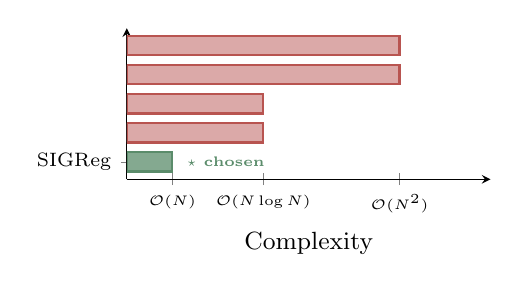
\begin{tikzpicture}
\begin{axis}[
  width=6.2cm, height=3.5cm,
  xbar, bar width=7pt, bar shift=0pt,
  xlabel={Complexity}, xlabel style={font=\small},
  symbolic y coords={SIGReg, Anderson-D., Cramér-vM, KL Div., MMD},
  ytick=data, yticklabel style={font=\scriptsize},
  xticklabel style={font=\tiny},
  xmin=0, xmax=4,
  xtick={0.5,1.5,3.0},
  xticklabels={$\mathcal{O}(N)$,$\mathcal{O}(N\log N)$,$\mathcal{O}(N^2)$},
  grid=none, axis x line=bottom, axis y line=left,
  enlarge y limits=0.15,
]
  \addplot[fill=mgood!75, draw=mgood, line width=0.8pt] coordinates
    {(0.5,SIGReg)};
  \addplot[fill=mbad!50, draw=mbad, line width=0.8pt] coordinates
    {(1.5,Anderson-D.) (1.5,Cramér-vM) (3,KL Div.) (3,MMD)};
  \node[mgood, font=\tiny\bfseries, anchor=west] at (axis cs:0.55,SIGReg) {$\star$ chosen};
\end{axis}
\end{tikzpicture}

\column{0.44\textwidth}
\vspace{0.3em}

\begin{badbox}
\footnotesize \textbf{MMD} (Maximum Mean Discrepancy): chứng minh được nhưng $\mathcal{O}(N^2)$ — không thể mở rộng tốt.
\end{badbox}

\vspace{0.4em}
\begin{badbox}
\footnotesize \textbf{KL Divergence:} gradient không ổn định khi $p\approx 0$, không differentiable.
\end{badbox}

\vspace{0.4em}
\begin{badbox}
\footnotesize \textbf{Test multivariate chuẩn} (BHEP, Mardia): đều $\mathcal{O}(N^2)$ — không thể dùng với mini-batch.
\end{badbox}

\vspace{0.5em}
\begin{accentbox}
\footnotesize \textbf{Giải pháp:} Phân rã bài toán $K$-chiều thành $M$ bài toán 1D độc lập qua random projection.
\end{accentbox}

\end{columns}

\end{frame}


% ─── [BATCH 2] 3 families — Moments unstable ─────────────────────────────────
\begin{frame}{Họ Test 1: Moments — Mạnh Nhưng Gradient Explode}

\begin{columns}[T]
\column{0.50\textwidth}

\textbf{Extended Jarque-Bera (EJB)} đo độ lệch khỏi Gaussian bằng cách gom \textbf{4 thống kê mô tả} (mean, variance, skewness, kurtosis) vào một score duy nhất.

\vspace{0.3em}
Score càng lớn $\rightarrow$ phân phối càng sai lệch so với $\mathcal{N}(0,1)$.

\vspace{0.5em}
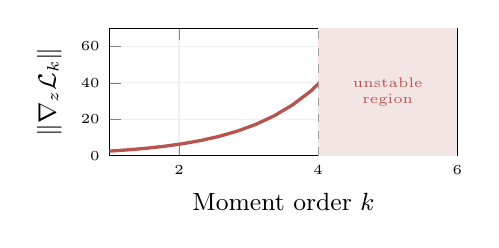
\begin{tikzpicture}
\begin{axis}[
  width=6.0cm, height=3.2cm,
  xlabel={Moment order $k$},
  ylabel={$\|\nabla_z \mathcal{L}_k\|$},
  xlabel style={font=\small}, ylabel style={font=\small},
  tick label style={font=\tiny},
  xmin=1, xmax=6, ymin=0, ymax=70,
  grid=major, grid style={mgray!15},
]
  \addplot[mbad, very thick, domain=1:6, samples=20] {2.5^x};
  \fill[mbad!15] (axis cs:4,0) rectangle (axis cs:6,70);
  \node[mbad, font=\tiny, align=center] at (axis cs:5, 35)
    {unstable\\region};
  \draw[mgray, dashed] (axis cs:4,0) -- (axis cs:4,70);
\end{axis}
\end{tikzpicture}


\column{0.46\textwidth}
\vspace{0.3em}

\begin{badbox}
\footnotesize\textbf{Định lý 3.} Với $K$ moment hữu hạn, điểm cực tiểu \emph{không phải là duy nhất}: nhiều phân phối khác nhau đều có thể có cùng $K$ moment đầu như Gaussian.
\end{badbox}

\vspace{0.5em}
\textbf{Vấn đề nan giải:} thêm nhiều moment hơn không giải quyết được vấn đề mà còn tạo ra vấn đề mới.

\vspace{0.5em}
\begin{tabular}{@{}lll@{}}
\toprule
 & $K$ nhỏ & $K$ lớn \\
\midrule
Nhận diện & \textcolor{mbad}{yếu} — nhiều & \textcolor{mgood}{mạnh} \\
& shortcut & \\
Gradient & \textcolor{mgood}{ổn định} & \textcolor{mbad}{explode} theo \\
& & hàm mũ \\
\bottomrule
\end{tabular}

\vspace{0.6em}
\begin{badbox}
\footnotesize\textbf{Không thể có cả hai:} tăng $K$ để nhận diện tốt hơn thì gradient bùng nổ → quá trình huấn luyện mất ổn định.
\end{badbox}

\end{columns}
\end{frame}


% ─── [BATCH 2] CDF family ────────────────────────────────────────────────────
\begin{frame}{Họ Test 2: CDF — Chính Xác Nhưng Không Differentiable}

\vspace{0.4em}
Họ test CDF đo khoảng cách giữa hai hàm phân bố tích luỹ. Tuy nhiên, việc tính toán thực nghiệm yêu cầu thao tác \textbf{sắp xếp} dữ liệu, gây ra hai hạn chế chí mạng cho học sâu:

\vspace{1.2em}
\begin{columns}[T]
\column{0.48\textwidth}
\begin{center}
\textcolor{mbad}{\textbf{\large \xmark\ Vấn đề 1: Non-parallel}}

\vspace{0.8em}
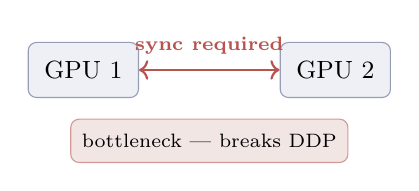
\begin{tikzpicture}[every node/.style={font=\scriptsize}]
  \node[pbox, minimum width=1.4cm, minimum height=0.7cm, font=\small]
    (g1) at (0, 0) {GPU 1};
  \node[pbox, minimum width=1.4cm, minimum height=0.7cm, font=\small]
    (g2) at (3.2, 0) {GPU 2};
  \draw[<->, thick, mbad] (g1.east) -- (g2.west)
    node[midway, above=2pt, font=\scriptsize\bfseries, mbad]{sync required};
  \node[rbox, minimum width=3.4cm, minimum height=0.55cm, font=\scriptsize, inner sep=4pt]
    at (1.6, -0.9) {bottleneck — breaks DDP};
\end{tikzpicture}

\vspace{0.8em}
\footnotesize Multi-GPU phải đồng bộ hóa toàn bộ dữ liệu trước khi sắp xếp $\Rightarrow$ tạo ra nút thắt cổ chai nghiêm trọng.
\end{center}

\column{0.48\textwidth}
\begin{center}
\textcolor{mbad}{\textbf{\large \xmark\ Vấn đề 2: Non-differentiable}}

\vspace{0.8em}
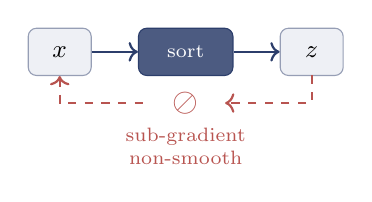
\begin{tikzpicture}[every node/.style={font=\scriptsize}]
  \node[pbox, minimum width=0.8cm, minimum height=0.6cm] (xn) at (0,0) {$x$};
  \node[darkbox, minimum width=1.2cm, minimum height=0.6cm, font=\scriptsize]
    (srt) at (1.6,0) {sort};
  \node[pbox, minimum width=0.8cm, minimum height=0.6cm] (zn) at (3.2,0) {$z$};
  \draw[arr] (xn)--(srt);
  \draw[arr] (srt)--(zn);
  
  \draw[<-, dashed, mbad, thick] (xn.south) -- (0,-0.65) -- (1.1,-0.65);
  \node[mbad, font=\large\bfseries] at (1.6,-0.65) {$\oslash$};
  \draw[->, dashed, mbad, thick] (3.2,-0.3) -- (3.2,-0.65) -- (2.1,-0.65);
  \node[mbad, font=\scriptsize, align=center] at (1.6,-1.2)
    {sub-gradient\\non-smooth};
\end{tikzpicture}

\vspace{0.8em}
\footnotesize Cần differentiable sort relaxation $\Rightarrow$ sinh thêm siêu tham số và sai số xấp xỉ.
\end{center}
\end{columns}

\vspace{1.5em}
\takeaway{Hạn chế cốt lõi của CDF: Phép toán sắp xếp bẻ gãy tính toán song song và triệt tiêu luồng gradient}
\end{frame}


% ─── [BATCH 2] Epps-Pulley (ECF) ─────────────────────────────────────────────
\begin{frame}{Họ Test 3: ECF — Stable, Scalable, Provable}

\vspace{0.2em}
\textbf{Epps-Pulley (EP) test} so sánh phân phối qua \textbf{miền tần số (ECF)}: tính trung bình các sóng $e^{itx}$.

\vspace{0.8em}
\begin{columns}[T]
\column{0.48\textwidth}

Vì $|e^{itx}| = 1$, giá trị ECF luôn ổn định.

\vspace{0.8em}
\begin{center}
\begin{tikzpicture}
\begin{axis}[
  width=5.2cm, height=3.0cm,
  xlabel={$t$ (tần số)}, ylabel={CF},
  xlabel style={font=\small}, ylabel style={font=\small},
  tick label style={font=\tiny},
  xmin=-5, xmax=5, ymin=-0.3, ymax=1.2,
  grid=major, grid style={mgray!15},
  legend pos=outer north east,
  legend style={font=\tiny, draw=none, fill=mgray!5},
]
  \addplot[mprimary, very thick, domain=-5:5, samples=60]
    {exp(-x^2/2)};
  \addlegendentry{Target $\phi(t)$}
  \addplot[maccent, thick, domain=-5:5, samples=80]
    {exp(-x^2/2) + 0.22*sin(deg(3.5*x))*exp(-x^2/2.2) + 0.08*cos(deg(7*x))*exp(-x^2/3)};
  \addlegendentry{Empirical $\hat\phi_X(t)$}
  % highlight gap region
  \addplot[fill=mbad!12, draw=none, domain=-3.5:3.5, samples=80]
    {exp(-x^2/2) + 0.22*sin(deg(3.5*x))*exp(-x^2/2.2) + 0.08*cos(deg(7*x))*exp(-x^2/3)}
    \closedcycle;
  \addplot[fill=white, draw=none, domain=-3.5:3.5, samples=80]
    {exp(-x^2/2)} \closedcycle;
  \node[font=\tiny, mgray, align=center] at (axis cs:2.8, 0.5) {gap\\$= EP$};
\end{axis}
\end{tikzpicture}
\end{center}

\column{0.48\textwidth}
\vspace{0.2em}

\textcolor{mgood}{\textbf{\large \checkmark\ Differentiable}}\\[2pt]
\footnotesize Gradient tự nhiên từ trung bình, không cần phép \emph{sort}.

\vspace{0.6em}
\textcolor{mgood}{\textbf{\large \checkmark\ $\mathcal{O}(N)$ \& DDP-friendly}}\\[2pt]
\footnotesize Song song hoá dễ dàng qua \texttt{all\_reduce}.

\vspace{0.6em}
\begin{primarybox}
\footnotesize \textbf{Định lý 4: Bounded Gradient}\\[2pt]
Gradient luôn \textbf{bị chặn an toàn} $\leq 4\sigma^2/N$ $\Rightarrow$ loại bỏ rủi ro exploding gradient.
\end{primarybox}

\end{columns}

\vspace{1.0em}
\takeaway{$|e^{itx}|=1$: Chìa khoá cho một hàm Loss 100\% song song hoá và siêu ổn định}
\end{frame}


% ─── Slide 7: SIGReg ─────────────────────────────────────────────────────────
\begin{frame}{SIGReg: Đưa Embedding Về $\mathcal{N}(0,I)$ Ở Chi Phí $\mathcal{O}(N)$}

\begin{columns}[T]
\column{0.52\textwidth}

\textbf{Vấn đề:} Test $P_\theta \stackrel{?}{=} \mathcal{N}(0,I)$ trong $K$-chiều tốn $\mathcal{O}(N^2)$.

\vspace{0.4em}
\textbf{Giải pháp — Cramér-Wold Sketching:}

Chiếu xuống $M$ hướng ngẫu nhiên $\mathbf{u} \in \mathbb{S}^{K-1}$:
\[
  X \stackrel{d}{=} Y \iff \langle \mathbf{u}, X\rangle \stackrel{d}{=} \langle \mathbf{u}, Y\rangle,\;\forall \mathbf{u}
\]

\vspace{0.4em}
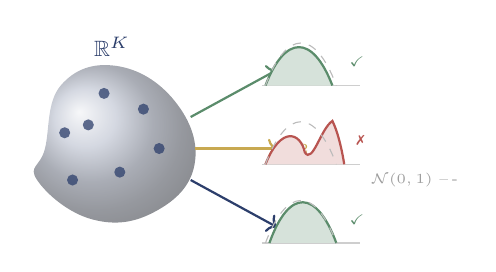
\begin{tikzpicture}[every node/.style={font=\scriptsize}]
  %% ── Blob K-dim ──
  \shade[ball color=mprimary!45, opacity=0.6]
    plot[smooth cycle, tension=0.72] coordinates {
      (0.15,0.3)(0.35,1.1)(1.05,1.35)(1.8,0.9)
      (2.05,0.1)(1.55,-0.5)(0.75,-0.6)(0.05,-0.1)
    };
  \foreach \px/\py in {0.4/0.5, 0.9/1.0, 1.4/0.8, 1.6/0.3, 1.1/0.0, 0.5/-0.1, 0.7/0.6}{
    \fill[mprimary, opacity=0.75] (\px,\py) circle (2pt);
  }
  \node[mprimary, font=\footnotesize\bfseries, above] at (1.0,1.35) {$\mathbb{R}^K$};

  %% ── 3 projection arrows ──
  \draw[->, thick, mgood]   (2.0,0.7) -- (3.1,1.3)  node[right, font=\tiny, mgood]{$\mathbf{u}_1$};
  \draw[->, thick, maccent] (2.05,0.3) -- (3.1,0.3)  node[right, font=\tiny, maccent]{$\mathbf{u}_2$};
  \draw[->, thick, mprimary](2.0,-0.1) -- (3.1,-0.7) node[right, font=\tiny, mprimary]{$\mathbf{u}_M$};

  %% ── Histogram u1 — khớp ──
  \begin{scope}[xshift=3.5cm, yshift=1.1cm]
    \draw[mgray!50, thin] (-0.6,0)--(0.65,0);
    \fill[mgood!25] (-0.55,0) .. controls(-0.3,0.65) and (0.05,0.65) .. (0.3,0) -- cycle;
    \draw[mgood, thick] (-0.55,0) .. controls(-0.3,0.65) and (0.05,0.65) .. (0.3,0);
    \draw[mgray!70, dashed, thin] (-0.55,0) .. controls(-0.28,0.72) and (0.08,0.72) .. (0.35,0);
    \node[mgood, font=\tiny, right=1pt] at (0.35,0.3) {\checkmark};
  \end{scope}

  %% ── Histogram u2 — mismatch ──
  \begin{scope}[xshift=3.5cm, yshift=0.1cm]
    \draw[mgray!50, thin] (-0.6,0)--(0.65,0);
    \fill[mbad!20] (-0.55,0) .. controls(-0.35,0.5) and (-0.1,0.4).. (-0.05,0.15)
      .. controls(0.05,0.0) and (0.15,0.45).. (0.3,0.55)
      .. controls(0.4,0.35) and (0.45,0).. (0.45,0) -- cycle;
    \draw[mbad, thick] (-0.55,0) .. controls(-0.35,0.5) and (-0.1,0.4).. (-0.05,0.15)
      .. controls(0.05,0.0) and (0.15,0.45).. (0.3,0.55)
      .. controls(0.4,0.35) and (0.45,0).. (0.45,0);
    \draw[mgray!70, dashed, thin] (-0.55,0) .. controls(-0.28,0.72) and (0.08,0.72) .. (0.35,0);
    \node[mbad, font=\tiny, right=1pt] at (0.45,0.3) {\xmark};
  \end{scope}

  %% ── Histogram uM — khớp ──
  \begin{scope}[xshift=3.5cm, yshift=-0.9cm]
    \draw[mgray!50, thin] (-0.6,0)--(0.65,0);
    \fill[mgood!25] (-0.5,0) .. controls(-0.25,0.70) and (0.1,0.68) .. (0.35,0) -- cycle;
    \draw[mgood, thick] (-0.5,0) .. controls(-0.25,0.70) and (0.1,0.68) .. (0.35,0);
    \draw[mgray!70, dashed, thin] (-0.55,0) .. controls(-0.28,0.72) and (0.08,0.72) .. (0.35,0);
    \node[mgood, font=\tiny, right=1pt] at (0.35,0.3) {\checkmark};
  \end{scope}
  \node[mgray, font=\tiny, right=2pt] at (4.1,-0.1) {$\mathcal{N}(0,1)$ {\color{mgray}--\,-}};
\end{tikzpicture}

\column{0.45\textwidth}
\vspace{0.2em}

\textbf{Test 1D: Epps-Pulley (ECF)}
\[EP = N\!\int |\hat\phi_X(t) - \phi(t)|^2 w(t)\,dt\]

$\hat\phi_X(t) = \tfrac{1}{N}\sum e^{itX_j}$ — luôn nằm trong $[-1,1]$.

\vspace{0.4em}
\begin{goodbox}
\footnotesize \textbf{Định lý 4:} Gradient EP bị chặn bởi $\frac{4\sigma^2}{N}$ — không bao giờ explode.
\end{goodbox}

\vspace{0.4em}
\begin{primarybox}
\footnotesize \textbf{SIGReg} = trung bình EP trên $M$ hướng ngẫu nhiên.\\[2pt]
$\mathcal{O}(N)$ · differentiable · DDP-friendly.
\end{primarybox}

\vspace{0.4em}
\begin{accentbox}
\footnotesize $M = 16$ hướng đủ nhờ tính trơn của DNN + SGD resampling tích lũy.
\end{accentbox}

\end{columns}

\end{frame}


% ─── [BATCH 2] SIGReg definition + code ─────────────────────────────────────
\begin{frame}[fragile]{SIGReg: Định Nghĩa Chính Thức và Cài đặt}

\begin{columns}[T]
\column{0.50\textwidth}

\begin{accentbox}
\footnotesize\textbf{Định nghĩa 2 — SIGReg}
\[
  \mathrm{SIGReg}_T(\mathbb{A},\{f_\theta(\mathbf{x}_n)\})
  \triangleq \frac{1}{|\mathbb{A}|}\sum_{\mathbf{a}\in\mathbb{A}}
  T\!\left(\{\mathbf{a}^\top f_\theta(\mathbf{x}_n)\}_{n=1}^N\right)
\]
$\mathbb{A}=\{\mathbf{a}_1,\ldots,\mathbf{a}_M\}$: tập hướng ngẫu nhiên trên $\mathbb{S}^{K-1}$.\\
$T$ được chọn là Epps-Pulley.
\end{accentbox}

\vspace{0.5em}
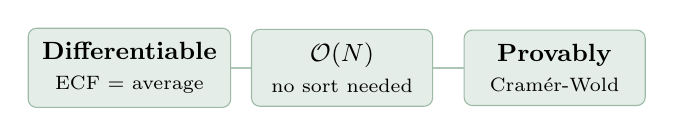
\begin{tikzpicture}[every node/.style={font=\small}]
  \node[gbox, minimum width=2.3cm, minimum height=0.8cm, align=center] (d) at (0,0)
    {\textbf{Differentiable}\\ \scriptsize ECF = average};
  \node[gbox, minimum width=2.3cm, minimum height=0.8cm, align=center] (s) at (2.7,0)
    {\textbf{$\mathcal{O}(N)$}\\ \scriptsize no sort needed};
  \node[gbox, minimum width=2.3cm, minimum height=0.8cm, align=center] (p) at (5.4,0)
    {\textbf{Provably}\\ \scriptsize Cramér-Wold};
  \draw[thick, mgood!50] (d.east)--(s.west);
  \draw[thick, mgood!50] (s.east)--(p.west);
\end{tikzpicture}

\vspace{0.3em}
\textbf{Tại sao average thay vì max?}\\
Max $\Rightarrow$ gradient sparse (chỉ 1 hướng được update). Average $\Rightarrow$ gradient dense, quá trình huấn luyện ổn định hơn.

\column{0.46\textwidth}
\vspace{0.3em}

\textbf{PyTorch — 50 dòng:}

\vspace{0.2em}
\begin{mdframed}[
  topline=false,bottomline=false,rightline=false,
  linewidth=2pt,linecolor=mprimary!50,
  backgroundcolor=mdark!5,
  innerleftmargin=6pt,innerrightmargin=4pt,
  innertopmargin=4pt,innerbottommargin=4pt
]
\tiny\ttfamily
\begin{lstlisting}[language=Python,basicstyle=\tiny\ttfamily]
def SIGReg(x, global_step, M=1024):
    g = torch.Generator(device=x.device)
    g.manual_seed(global_step)  # sync GPUs
    A = torch.randn(x.size(1), M, generator=g)
    A /= A.norm(p=2, dim=0)    # unit vectors
    t = torch.linspace(-5, 5, 17)
    phi = torch.exp(-0.5 * t**2)
    x_t = (x @ A).unsqueeze(-1) * t
    ecf_r = x_t.cos().mean(0)
    ecf_i = x_t.sin().mean(0)
    err = (ecf_r-phi).square() + ecf_i.square()
    return (err * phi).mean() * x.size(0)
\end{lstlisting}
% def SIGReg(x, global\_step, M=1024):\\
% \quad g = torch.Generator(device=x.device)\\
% \quad g.manual\_seed(global\_step) \# sync GPUs\\
% \quad A = torch.randn(x.size(1), M, generator=g)\\
% \quad A /= A.norm(p=2, dim=0) \# unit vectors\\
% \quad t = torch.linspace(-5, 5, 17)\\
% \quad phi = torch.exp(-0.5 * t**2) \# N(0,1) CF\\
% \quad x\_t = (x @ A).unsqueeze(-1) * t\\
% \quad ecf\_r = x\_t.cos().mean(0)\\
% \quad ecf\_i = x\_t.sin().mean(0)\\
% \quad err = (ecf\_r-phi).square() + ecf\_i.square()\\
% \quad return (err * phi).mean() * x.size(0)
\end{mdframed}

\end{columns}
\end{frame}


% ─── Slide 8: LeJEPA loss ─────────────────────────────────────────────────────
\begin{frame}{LeJEPA: Một Công Thức, Một Siêu Tham Số}

\begin{center}
\[
  \mathcal{L}_{\rm LeJEPA}
  = \underbrace{(1-\lambda)\cdot\mathcal{L}_{\rm pred}}_{\displaystyle\text{views phải agree}}
  \;+\;
  \underbrace{\lambda\cdot\text{SIGReg}}_{\displaystyle\text{push về }\mathcal{N}(\mathbf{0},I)}
\]
\end{center}

\vspace{-0.3em}
\begin{columns}[c]
\column{0.49\textwidth}

\vspace{-0.8em}
\begin{center}
\hspace*{-0.8em}\resizebox{1.10\linewidth}{!}{
\begin{tikzpicture}[
    every node/.style={font=\small},
    viewbox/.style={pbox, minimum width=1.6cm, minimum height=0.6cm, font=\scriptsize, align=center},
    encbox/.style={darkbox, minimum width=1.6cm, minimum height=3.6cm, align=center},
    projbox/.style={pbox, fill=mprimary!10, draw=mprimary, minimum width=1.6cm, minimum height=2.6cm, align=center},
    lossbox/.style={rectangle, draw, rounded corners=3pt, thick, align=center, minimum height=0.7cm, font=\scriptsize, inner sep=4pt}
  ]
  
  % Inputs
  \node[font=\small\bfseries, draw=mgray, rounded corners, inner sep=4pt, text=mprimary] (img) at (0, 0) {Image $\mathbf{x}$};
  
  % Views
  \node[viewbox] (v1) at (3, 1.8) {view 1\\(global)};
  \node[viewbox] (v2) at (3, 0.6) {view 2\\(global)};
  \node[font=\small, mgray] (vd) at (3, -0.4) {$\vdots$};
  \node[viewbox] (v8) at (3, -1.4) {view 8\\(local)};
  
  \draw[->, thick, mgray] (img) |- (v1) node[pos=0.75, above=0pt, font=\tiny] {aug};
  \draw[->, thick, mgray] (img) |- (v2) node[pos=0.75, above=0pt, font=\tiny] {aug};
  \draw[->, thick, mgray] (img) |- (v8) node[pos=0.75, above=0pt, font=\tiny] {aug};
  
  % Encoder
  \node[encbox] (enc) at (5.8, 0.2) {Encoder\\$f_\theta$\\ \tiny(bất kỳ)};
  \draw[->, thick, mgray] (v1) -- (v1 -| enc.west);
  \draw[->, thick, mgray] (v2) -- (v2 -| enc.west);
  \draw[->, thick, mgray] (v8) -- (v8 -| enc.west);
  
  % Projector
  \node[projbox] (proj) at (8.3, 0.2) {Proj Head\\ \tiny(3-layer MLP)};
  \draw[->, thick, mgray] (enc) -- (proj);
  
  % z
  \node[circle, draw=mprimary, thick, fill=white, inner sep=1.5pt, font=\normalsize\bfseries, text=mprimary] (z) at (10.6, 0.2) {$\mathbf{z}$};
  \draw[->, thick, mprimary] (proj) -- (z);
  
  % Losses
  \node[lossbox, draw=mbad, fill=mbad!10, text=mbad!80!black] (inv) at (7.4, -2.4) {\textbf{Invariance Loss}\\$\mathcal{L}_{\rm pred} \; (\mathbf{z}_v \approx \boldsymbol{\mu})$};
  \node[lossbox, draw=mgood, fill=mgood!10, text=mgood!80!black] (sig) at (10.6, -2.4) {\textbf{SIGReg Loss}\\$\mathbf{z} \sim \mathcal{N}(0, I)$};
  
  \draw[->, mbad, thick, rounded corners] (z.south) |- (8.8, -1.4) -| (inv.north);
  \draw[->, mgood, thick] (z.south) -- (sig.north);
  
\end{tikzpicture}
}
\end{center}

\column{0.49\textwidth}

\vspace{0.2em}
\begin{tabular}{@{}lccc@{}}
\toprule
 & DINO & I-JEPA & \textbf{LeJEPA} \\
\midrule
Lý thuyết         & \textcolor{mbad}{\xmark} & \textcolor{mbad}{\xmark} & \textcolor{mgood}{\textbf{\cmark}} \\
\# hyperparams    & $\geq$7 & $\geq$5 & \textbf{1\ ($\lambda$)} \\
Architecture      & ViT  & ViT   & \textbf{Any} \\
Stop-gradient     & cần  & cần   & \textbf{không} \\
Teacher-student   & cần  & cần   & \textbf{không} \\
Core code (lines) & 1000+ & 500+ & \textbf{$\approx$50} \\
\bottomrule
\end{tabular}

\end{columns}

\takeaway{1 loss · 1 hyperparameter · 0 heuristic · lý thuyết từ first principles}

\end{frame}


% ─── [BATCH 3] Curse of dimensionality ───────────────────────────────────────
% \begin{frame}{SIGReg Vượt Qua Curse of Dimensionality}

% \begin{columns}[T]
% \column{0.50\textwidth}

% \textbf{Định lý 5 (Unified Error Bound):}\\[4pt]
% Khoảng cách thực sự giữa không gian Latent và $\mathcal{N}(0,I)$ luôn bị chặn trên bởi $\mathcal{O}\big(M^{-\frac{2\alpha}{K-1}}\big)$, với $\alpha$ là độ trơn (smoothness) của dữ liệu.

% \vspace{0.6em}
% \begin{tikzpicture}
% \begin{axis}[
%   width=5.2cm, height=3.2cm,
%   xlabel={$M$ (số hướng, log-scale)}, ylabel={Sai số kỳ vọng},
%   xmode=log,
%   xlabel style={font=\small}, ylabel style={font=\small},
%   tick label style={font=\tiny},
%   xmin=16, xmax=2048, ymin=0, ymax=1200,
%   grid=major, grid style={mgray!15},
%   legend pos=outer north east,
%   legend style={font=\tiny, draw=none, fill=mgray!5, inner sep=2pt, nodes={inner sep=1pt}},
% ]
%   \addplot[mbad, thick, domain=16:2048, samples=30]
%     {1100*exp(-x/800)};
%   \addlegendentry{Fixed $\mathbb{A}$}
%   \addplot[mgood, very thick, domain=16:2048, samples=30]
%     {1100*exp(-x/120)};
%   \addlegendentry{Resampled (SGD)}
% \end{axis}
% \end{tikzpicture}

% \column{0.46\textwidth}
% \vspace{0.3em}

% \textbf{Hai lý do SIGReg thắng curse:}

% \vspace{0.4em}
% \begin{primarybox}
% \footnotesize \textbf{1. Sobolev smoothness $\alpha$:} DNN tự nhiên smooth (BatchNorm, Dropout, weight decay) $\Rightarrow$ $\alpha$ lớn $\Rightarrow$ tốc độ hội tụ $|\mathbb{A}|^{-2\alpha/(K-1)}$ nhanh $\Rightarrow$ $M=\mathcal{O}(K)$ là đủ.
% \end{primarybox}

% \vspace{0.4em}
% \begin{primarybox}
% \footnotesize \textbf{2. SGD resampling:} Mỗi mini-batch lấy mẫu lại $M$ hướng mới $\Rightarrow$ sau $T$ bước huấn luyện, số hướng tích lũy $=M\times T$ $\Rightarrow$ coverage tăng miễn phí.
% \end{primarybox}

% \vspace{0.4em}
% \begin{goodbox}
% \footnotesize $M=16$ hướng mỗi bước đủ để match $K=2048$-dim embedding, nhờ resampling compounding.
% \end{goodbox}

% \end{columns}
% \end{frame}


% ─── [BATCH 3] Lambda tradeoff ────────────────────────────────────────────────
\begin{frame}{$\lambda$: Nút Điều Chỉnh Duy Nhất}

\begin{columns}[T]
\column{0.50\textwidth}

\begin{tikzpicture}[every node/.style={font=\small}, scale=0.9]
  % Spectrum
  \draw[->, thick, mgray!60] (0,0) -- (6.5,0) node[right,font=\tiny]{$\lambda$};

  % lambda=0
  \draw[thick,mgray] (0.3,0.15)--(0.3,-0.15);
  \node[font=\tiny,below=2pt] at (0.3,0) {$0$};
  \node[mbad, font=\tiny, align=center] at (0.3, 1.1)
    {Pure Pred.\\Collapse};
  \fill[mbad!20] (0.3,0.45) circle (0.25cm);
  \fill[mbad] (0.3,0.45) circle (0.05cm);

  % lambda=1
  \draw[thick,mgray] (6.2,0.15)--(6.2,-0.15);
  \node[font=\tiny,below=2pt] at (6.2,0) {$1$};
  \node[mbad, font=\tiny, align=center] at (6.2, 1.1)
    {Pure SIGReg\\Uniform};
  \foreach \px/\py in {5.95/0.5, 6.25/0.35, 6.0/0.3, 6.3/0.55, 6.15/0.45}{
    \fill[mbad!60] (\px,\py) circle (0.04cm);
  }

  % sweet spot
  \draw[thick, mgood, line width=1.5pt] (2.2,0.15)--(2.2,-0.15);
  \node[font=\tiny,below=2pt,mgood] at (2.2,0) {$0.05$};
  \node[mgood, font=\small\bfseries, align=center] at (2.2, 1.2)
    {Sweet spot};
  \fill[mgood!20] (2.2,0.5) circle (0.32cm);
  \foreach \px/\py in {2.05/0.6, 2.35/0.42, 2.0/0.42, 2.38/0.6, 2.2/0.5}{
    \fill[mgood!70] (\px,\py) circle (0.04cm);
  }

  % brace
  \draw[decorate, decoration={brace, amplitude=4pt}, mgood!70, thick]
    (3.2,-0.45) -- (1.3,-0.45)
    node[midway,below=4pt,font=\tiny,mgood]{vùng ổn định};
\end{tikzpicture}

\vspace{0.3em}
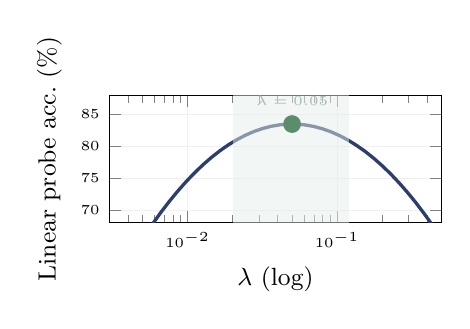
\begin{tikzpicture}
\begin{axis}[
  width=5.8cm, height=3.2cm,
  xlabel={$\lambda$ (log)}, ylabel={Linear probe acc.\ (\%)},
  xmode=log, xlabel style={font=\small}, ylabel style={font=\small},
  tick label style={font=\tiny},
  xmin=0.003, xmax=0.5, ymin=68, ymax=88,
  grid=major, grid style={mgray!15},
]
  \addplot[mprimary, very thick, domain=0.003:0.5, samples=40]
    {83.5 - 18*(log10(x) - log10(0.05))^2};
  \addplot[mark=*, mgood, mark size=3pt] coordinates {(0.05,83.5)}
    node[above=3pt,font=\tiny,mgood]{$\lambda=0.05$};
  \fill[mgood!15,opacity=0.5] (axis cs:0.02,68) rectangle (axis cs:0.12,88);
\end{axis}
\end{tikzpicture}

\column{0.46\textwidth}
\vspace{0.3em}

\begin{primarybox}
\footnotesize \textbf{Thiết lập mặc định khuyên dùng:}\\[3pt]
$\lambda = 0.05$\\
$V_g=2$ global views, $V_l=6$ local\\
batch size $\geq 128$\\
$M=1024$ slices\\
17 quadrature points, $t\in[-5,5]$
\end{primarybox}

\vspace{0.5em}
\begin{goodbox}
\footnotesize $\lambda$ robust trên dải rộng (Figure 8 trong paper: stable $\lambda\in[0.01, 0.1]$) — không cần grid search tỉ mỉ.
\end{goodbox}

\vspace{0.5em}
\textbf{Scaling law với số views:} peak $\lambda$ tỉ lệ thuận với $V$ — nếu tăng views thì tăng $\lambda$ tương ứng.

\end{columns}
\end{frame}


% ─── [BATCH 3] LeJEPA vs prior + VICReg relation ─────────────────────────────
\begin{frame}{LeJEPA Generalizes VICReg — Và Giải Thích Tại Sao VICReg Bị Hạn Chế}

\begin{columns}[T]
\column{0.48\textwidth}

\textbf{Sự kết nối lý thuyết:}\\[4pt]
Nếu thay thế hàm Test $T$ trong SIGReg bằng \textbf{hàm tính Moment} (chỉ đo trung bình và phương sai), SIGReg sẽ hội tụ chính xác về \textbf{VICReg}.

\vspace{0.8em}
\begin{tikzpicture}[every node/.style={font=\footnotesize}, scale=0.95]
  \node[darkbox, minimum width=3.4cm, minimum height=0.65cm, align=center]
    (lj) at (0,0) {\textbf{LeJEPA}\\(Framework Tổng Quát)};

  \node[gbox, minimum width=3.4cm, minimum height=0.65cm, align=center]
    (ep) at (0,-1.4) {$T$ = \textbf{Epps-Pulley}\\(Khuyên dùng: Toàn diện)};

  \node[pbox, minimum width=3.4cm, minimum height=0.65cm, align=center]
    (vc) at (0,-2.8) {$T$ = \textbf{Moments}\\$\Rightarrow$ Trở thành \textbf{VICReg}};

  \node[rbox, minimum width=3.4cm, minimum height=0.65cm, align=center]
    (jb) at (0,-4.2) {$T$ = \textbf{Jarque-Bera}\\(Không ổn định)};

  \draw[arr, mgray] (lj)--(ep); 
  \draw[darr, mgray] (lj.west) to[out=180,in=180] node[left=1pt, font=\tiny, align=right]{case\\đặc biệt} (vc.west);
  \draw[darr, mgray] (lj.west) to[out=180,in=180] node[left=1pt, font=\tiny, align=right]{case\\đặc biệt} (jb.west);
\end{tikzpicture}

\column{0.48\textwidth}
\vspace{0.3em}

\textbf{Tại sao VICReg không đủ?}

\vspace{0.3em}
\begin{badbox}
\footnotesize \textbf{Định lý 3:} VICReg chỉ đối chiếu 2 moment đầu ($\hat\mu, \hat\sigma^2$) $\Rightarrow$ Dễ dính \textbf{shortcut} (nhiều phân phối khác nhau có cùng $\hat\mu, \hat\sigma^2$).\\[2pt]
$\Rightarrow$ Phải chắp vá bằng các heuristic phụ để tránh sụp đổ.
\end{badbox}

\vspace{0.6em}
\begin{goodbox}
\footnotesize \textbf{SIGReg:} Ràng buộc \textbf{toàn bộ} đặc trưng phân phối qua ECF $\Rightarrow$ Đảm bảo hội tụ tuyệt đối (Cramér-Wold).
\end{goodbox}

\vspace{0.6em}
\begin{accentbox}
\footnotesize \textbf{Kết luận:} VICReg thực chất là một phiên bản giới hạn và thiếu chặt chẽ của LeJEPA.
\end{accentbox}

\end{columns}
\end{frame}


% ─── SECTION DIVIDER ──────────────────────────────────────────────────────────
\section{Kết quả}


% % ─── Slide 9: Training loss + in-domain ──────────────────────────────────────
% \begin{frame}{Hai Kết Quả Nổi Bật}

% \begin{columns}[T]
% \column{0.48\textwidth}

% \textbf{Loss huấn luyện dự báo downstream performance}

% \vspace{0.2em}
% \begin{tikzpicture}
% \begin{axis}[
%   width=5.8cm, height=4.0cm,
%   xlabel={Test acc.\ (\%)},
%   ylabel={Loss huấn luyện},
%   ymode=log,
%   xlabel style={font=\small},
%   ylabel style={font=\small},
%   tick label style={font=\tiny},
%   xmin=0, xmax=72,
%   ymin=0.4, ymax=12,
%   grid=major, grid style={mgray!15},
% ]
%   % Simulated scatter (trend from paper)
%   \addplot[only marks, mark=*, mark size=1.6pt,
%            mprimary!60, opacity=0.75]
%     coordinates {
%       (5,9.5)(10,7.2)(15,5.5)(18,4.2)(22,3.4)
%       (27,2.6)(32,2.1)(38,1.7)(44,1.4)(50,1.1)
%       (56,0.9)(62,0.75)(68,0.62)(8,8.5)(14,6.0)
%       (20,4.8)(25,3.0)(35,2.3)(42,1.85)(55,1.0)
%     };
%   \addplot[maccent, very thick, domain=3:70, samples=30]
%     {7.5*exp(-x/14)};
%   \node[font=\tiny, maccent, fill=white, inner sep=1pt]
%     at (axis cs:50, 2.8) {$\rho_s \approx 94\%$ Spearman};
% \end{axis}
% \end{tikzpicture}

% \column{0.48\textwidth}

% \textbf{In-domain SSL đánh bại frontier models}\\
% \footnotesize Galaxy10 (11K ảnh thiên hà):

% \vspace{0.2em}
% \begin{tikzpicture}
% \begin{axis}[
%   width=5.2cm, height=4.0cm,
%   xlabel={Số mẫu mỗi lớp},
%   ylabel={Accuracy (\%)},
%   xmode=log,
%   xlabel style={font=\small},
%   ylabel style={font=\small},
%   tick label style={font=\tiny},
%   xmin=0.8, xmax=250,
%   ymin=15, ymax=88,
%   grid=major, grid style={mgray!15},
%   legend pos=outer north east,
%   legend style={font=\tiny, draw=none, fill=mgray!5, inner sep=2pt, nodes={inner sep=1pt}},
% ]
%   \addplot[mgray!70, thick, mark=square*, mark size=1.5pt]
%     coordinates {(1,21)(2,22)(5,30)(10,36)(100,61)(180,68)};
%   \addlegendentry{DINOv2}
%   \addplot[mgray!50, thick, mark=triangle*, mark size=1.5pt, dashed]
%     coordinates {(1,25)(2,29)(5,37)(10,45)(100,70)(180,73)};
%   \addlegendentry{DINOv3}
%   \addplot[mgood, very thick, mark=*, mark size=2pt]
%     coordinates {(1,31)(2,38)(5,52)(10,61)(100,75)(180,78)};
%   \addlegendentry{LeJEPA}
% \end{axis}
% \end{tikzpicture}
% \end{columns}

% \vspace{0.4em}
% \begin{columns}[T]
% \column{0.48\textwidth}
% \begin{primarybox}
% \footnotesize Lần đầu trong SSL: loss huấn luyện \textbf{tương quan 94\%} với accuracy — chọn model không cần linear probe.
% \end{primarybox}

% \column{0.48\textwidth}
% \begin{goodbox}
% \footnotesize Domain-specific SSL $>$ frontier transfer — ngay cả khi chỉ có 11K samples.
% \end{goodbox}
% \end{columns}

% \end{frame}


% % ─── Slide 10: Scale ─────────────────────────────────────────────────────────
% \begin{frame}{Scale: 60+ Kiến Trúc, Không Collapse, SOTA}

% \begin{columns}[T]
% \column{0.46\textwidth}
% \vspace{0.2em}

% 50 models, 8 architecture families, ImageNet-10:

% \begin{tikzpicture}
% \begin{axis}[
%   width=5.6cm, height=4.2cm,
%   xlabel={Parameters (M)},
%   ylabel={Top-1 Acc.\ (\%)},
%   xlabel style={font=\small},
%   ylabel style={font=\small},
%   tick label style={font=\tiny},
%   xmin=1, xmax=20, ymin=90, ymax=96,
%   grid=major, grid style={mgray!15},
%   legend style={font=\tiny, at={(1.05,0.5)},
%                 anchor=west, draw=none},
% ]
%   \addplot[only marks, mark=*, mark size=2pt, mprimary!80]
%     coordinates {(6,92.5)(10,93.2)(14,93.8)(17,94.1)(19,94.5)};
%   \addlegendentry{ResNet}
%   \addplot[only marks, mark=square*, mark size=2pt, mgood]
%     coordinates {(5,92.9)(9,94.0)(13,94.6)(16,95.0)};
%   \addlegendentry{ViT}
%   \addplot[only marks, mark=triangle*, mark size=2pt, maccent!90]
%     coordinates {(3,91.5)(7,92.2)(11,92.8)(18,93.5)};
%   \addlegendentry{Khác}
%   \draw[<->, mbad, thick] (axis cs:1.2,91.5) -- (axis cs:1.2,95.0)
%     node[midway, left=1pt, font=\tiny, mbad]{3.5\%};
% \end{axis}
% \end{tikzpicture}

% \textcolor{mgood}{\textbf{Không collapse nào}} trong tất cả 50 models.

% \column{0.50\textwidth}
% \vspace{0.3em}

% \begin{accentbox}
% \footnotesize\bfseries ImageNet-1K · ViT-H/14 · 100 epochs:
% \begin{center}
% {\Huge\bfseries\color{mprimary} 79.0\%}\\[3pt]
% \small linear probe, frozen backbone
% \end{center}
% \end{accentbox}

% \vspace{0.4em}
% \begin{tabular}{@{}lrr@{}}
% \toprule
% Method & Params & Acc \\
% \midrule
% I-JEPA ViT-H (300ep) & 632M & 77.3\% \\
% LeJEPA ViT-L (100ep) & 304M & 78.2\% \\
% \textbf{LeJEPA ConvNeXt-H} & 660M & \textbf{79.0\%} \\
% \bottomrule
% \end{tabular}

% \vspace{0.4em}
% \begin{goodbox}
% \footnotesize 3$\times$ ít compute · model nhỏ hơn · vẫn SOTA.
% \end{goodbox}

% \end{columns}

% \end{frame}


% % ─── [BATCH 4] Ablation stability ────────────────────────────────────────────
% \begin{frame}{Ablation: LeJEPA Ổn Định Trên Mọi Siêu Tham Số}

% \begin{columns}[T]
% \column{0.50\textwidth}

% \textbf{Epps-Pulley hyperparameters} (ViT-L/14, ImageNet-1K, 100ep):

% \vspace{0.3em}
% \begin{tabular}{@{}ccrrrr@{}}
% \toprule
% Integ. & $M$ & \multicolumn{3}{c}{\# quad. points} \\
% \cmidrule(lr){3-5}
%  & & 5 & 17 & 41 \\
% \midrule
% $[-1,1]$ & 512  & 71.8 & 72.1 & 72.0 \\
% $[-3,3]$ & 512  & 74.0 & 74.2 & 74.0 \\
% $[-5,5]$ & 512  & 73.7 & \textbf{74.2} & 74.2 \\
% $[-5,5]$ & 2048 & 74.5 & \textbf{74.8} & 74.8 \\
% \bottomrule
% \end{tabular}

% \vspace{0.5em}
% \textbf{Register tokens:} không cần thiết.

% \vspace{0.2em}
% \begin{tabular}{@{}lrr@{}}
% \toprule
% reg\_tokens & $M=1024$ & $M=4096$ \\
% \midrule
% 0 & 75.14 & 75.61 \\
% 2 & 75.08 & 75.67 \\
% 8 & 75.23 & 75.84 \\
% \bottomrule
% \end{tabular}

% \column{0.46\textwidth}
% \vspace{0.3em}

% \textbf{So sánh vs DINO/I-JEPA:}

% \vspace{0.3em}
% \begin{tabular}{@{} >{\footnotesize}l >{\footnotesize\color{mbad}}c >{\footnotesize\color{mbad}}c >{\footnotesize\color{mgood}\bfseries}c @{}}
% \toprule
% \footnotesize Tiêu chí & \footnotesize DINO & \footnotesize I-JEPA & \footnotesize LeJEPA \\
% \midrule
% Anti-collapse   & EMA+sg  & sg+mask & Theorem \\
% \# Hyperparams  & $\geq$7 & $\geq$5 & 1 ($\lambda$) \\
% Complexity      & $\mathcal{O}(N)$ & $\mathcal{O}(N)$ & $\mathcal{O}(N)$ \\
% Architecture    & ViT     & ViT     & Any (60+) \\
% Loss corr.      & ${\sim}20\%$ & ${\sim}30\%$ & 94\% \\
% Core code       & 1000+   & 500+    & $\approx$50 \\
% \bottomrule
% \end{tabular}

% \vspace{0.5em}
% \begin{accentbox}
% \footnotesize Không có collapse nào trong tất cả 50+ models, không tinh chỉnh siêu tham số theo kiến trúc.
% \end{accentbox}

% \end{columns}
% \end{frame}


% % ─── [BATCH 4] Emergent semantics ────────────────────────────────────────────
\begin{frame}{Emergent Semantics: Không Supervision — Vẫn Học Được Cấu Trúc}

\begin{columns}[T]
\column{0.48\textwidth}

\textbf{PCA last-layer features} (ViT-L, ImageNet):

\vspace{0.6em}
\begin{tikzpicture}[every node/.style={font=\small}]
  %% Image placeholder (dog on grass)
  \node[inner sep=0pt, draw=mgray!40, thick, rounded corners=3pt,
        path picture={
          \node at (path picture bounding box.center) {
            \includegraphics[width=2.4cm, height=2.4cm]{dog.png}
          };
        }] 
    (img) at (0,0) {\phantom{\rule{2.4cm}{2.4cm}}};

  %% Arrow
  \draw[->, thick, mprimary] (1.35, 0) -- (1.65, 0)
    node[above=2pt, midway, font=\tiny\bfseries]{PCA};

  %% PCA visualization — color-coded regions
  \begin{scope}[xshift=3.0cm]
    % Sky/Trees (Cool)
    \fill[cyan!15, rounded corners=3pt] (-1.2,-1.2) rectangle (1.2,1.2);
    % Grass (Cool)
    \fill[teal!25, rounded corners=3pt] (-1.2,-1.2) rectangle (1.2,-0.1);
    
    % Dog silhouette (Warm)
    \fill[maccent!80, opacity=0.9]
      plot[smooth cycle] coordinates {
        (0, 0.8)     % head top
        (0.35, 0.4)  % right ear/shoulder
        (0.45, -0.6) % right paw
        (-0.45, -0.6)% left paw
        (-0.35, 0.4) % left ear/shoulder
      };

    % Outer border
    \draw[mgray!60, thick, rounded corners=3pt] (-1.2,-1.2) rectangle (1.2,1.2);

    % Labels
    \node[font=\bfseries\tiny, white, align=center] at (0, 0.1) {dog\\(warm)};
    \node[font=\bfseries\tiny, teal!80!black, align=center] at (-0.75, 0.6) {bg\\(cool)};
    \node[font=\bfseries\tiny, teal!80!black] at (0.0,-0.85) {ground (cool)};
  \end{scope}

  \node[font=\scriptsize, mgray, align=center] at (1.5, -1.6)
    {3 PC $\to$ RGB, không dùng nhãn};
\end{tikzpicture}

\vspace{0.8em}
\textbf{Video segmentation tự động:}\\[2pt]
Thresholding attention map của CLS token giúp mask đối tượng chính xác theo frame, \emph{temporal coherence} cực mượt.

\column{0.48\textwidth}

\begin{goodbox}
\footnotesize \textbf{Warm colors} (đỏ/cam): foreground objects — chó, két, mặt.\\[5pt]
\textbf{Cool colors} (xanh lam/lục): background — cỏ, trời, lá.\\[5pt]
$\Rightarrow$ Tự động phân tách cấu trúc mà không cần bất kỳ annotation nào!
\end{goodbox}

\vspace{0.6em}
\begin{accentbox}
\footnotesize Khi tối ưu đúng chuẩn \textbf{SIGReg}, cấu trúc ngữ nghĩa (semantic structure) của dữ liệu sẽ tự nổi lên một cách tự nhiên.
\end{accentbox}

\end{columns}

\vspace{0.8em}
\begin{primarybox}
\footnotesize \textbf{Lý do cốt lõi:} Mục tiêu $\mathcal{N}(0,I)$ ép mọi hướng trong không gian embedding đều phải chứa thông tin (maximum entropy) — triệt tiêu hoàn toàn hiện tượng dimensional collapse.
\end{primarybox}
\end{frame}

% ─── Impact: LeWorldModel ─────────────────────────────────────────────────────
\begin{frame}{Tác Động Thực Tế: Từ Lý Thuyết Đến LeWorldModel}

\begin{columns}[c]
\column{0.45\textwidth}

\begin{center}
\begin{tikzpicture}[every node/.style={font=\small, align=center}]

  %% LeJEPA Box
  \node[draw=mprimary, fill=mprimary!8, rounded corners=4pt, inner sep=6pt, text width=3.5cm, line width=1pt] 
    (lejepa) at (0, 0) {\textbf{LeJEPA}\\(\textit{Chỉ mã hóa tĩnh})\\\vspace{0.15cm}\scriptsize SIGReg Anti-collapse};

  %% LeWorldModel Box
  \node[draw=mgood, fill=mgood!8, rounded corners=4pt, inner sep=6pt, text width=3.5cm, line width=1pt] 
    (lewm) at (0, -2.8) {\textbf{LeWorldModel}\\(\textit{World Model động})\\\vspace{0.15cm}\scriptsize ViT Encoder + Predictor};

  %% Arrow down
  \draw[->, thick, mprimary] (lejepa.south) -- (lewm.north) node[midway, right, font=\scriptsize, mprimary]{Áp dụng};

  %% Results Boxes
  \node[draw=maccent, fill=maccent!8, rounded corners=3pt, inner sep=4pt, text width=1.5cm, font=\scriptsize, line width=0.8pt] 
    (res1) at (-1.3, -4.6) {\textbf{Planning}\\nhanh hơn\\$\mathbf{48\times}$};
    
  \node[draw=maccent, fill=maccent!8, rounded corners=3pt, inner sep=4pt, text width=1.5cm, font=\scriptsize, line width=0.8pt] 
    (res2) at (1.3, -4.6) {\textbf{Probing}\\Vật lý\\vượt trội};

  %% Arrows branching out safely
  \draw[->, thick, mgood] (lewm.south) -- (res1.north);
  \draw[->, thick, mgood] (lewm.south) -- (res2.north);

\end{tikzpicture}
\end{center}

\column{0.50\textwidth}
\textbf{LeWorldModel} (arXiv:2603.19312)

\vspace{0.3cm}
\begin{itemize}\small
  \setlength{\itemsep}{0.6em}
  \item[\textcolor{mgood}{\textbf{\cmark}}] \textbf{End-to-end từ pixels:} Không dùng pre-trained encoder hay stop-gradient.
  \item[\textcolor{mgood}{\textbf{\cmark}}] \textbf{Tối giản hóa:} Đúng \textbf{2 loss terms} (thay vì 7).
  \item[\textcolor{mgood}{\textbf{\cmark}}] \textbf{Planning vượt trội:} Nhanh hơn \textbf{48$\times$} foundation WMs.
  \item[\textcolor{mgood}{\textbf{\cmark}}] \textbf{Gọn nhẹ:} Chỉ 15M params, huấn luyện trên \textbf{1 GPU}.
\end{itemize}

\vspace{0.5cm}
\begin{accentbox}
\centering\small\itshape
"SIGReg enables the first stable end-to-end JEPA world model — no EMA, no stop-gradient, no reconstruction loss."
\end{accentbox}

\end{columns}

\end{frame}


% ─── Conclusion ───────────────────────────────────────────────────────────────
\begin{frame}[plain]
\begin{center}
\vspace{0.7cm}
{\Large\bfseries\color{mprimary} LeJEPA — Từ Heuristic Đến Lý Thuyết}

\vspace{0.5cm}
\begin{tikzpicture}[every node/.style={font=\small}, scale=0.88]
  \node[rbox, minimum width=2.8cm, minimum height=1.1cm, align=center]
    (old) at (0,0)
    {\textbf{Prior SSL}\\\small chắp vá thực nghiệm};

  \node[darkbox, minimum width=2.8cm, minimum height=1.1cm, align=center]
    (new) at (6.5,0)
    {\textbf{LeJEPA}\\\small từ nguyên lý nền tảng};

  \draw[->, very thick, mprimary, line width=2pt] (old) -- (new)
    node[midway, above=3pt, font=\small, mprimary]
      {Định lý + SIGReg};
\end{tikzpicture}

\vspace{0.55cm}
\begin{columns}[c]
\column{0.05\textwidth}
\column{0.90\textwidth}
\begin{itemize}\small
  \item[\textcolor{mgood}{\textbf{\cmark}}]
    \textbf{Lý thuyết:} Isotropic Gaussian là unique minimizer cho worst-case downstream risk
  \item[\textcolor{mgood}{\textbf{\cmark}}]
    \textbf{Phương pháp:} SIGReg — $\mathcal{O}(N)$, differentiable, bounded gradient
  \item[\textcolor{mgood}{\textbf{\cmark}}]
    \textbf{Thực nghiệm:} Đạt SOTA trên 60+ architectures, đánh bại DINOv2 in-domain
  \item[\textcolor{mgood}{\textbf{\cmark}}]
    \textbf{Tối giản:} Chỉ 1 hyperparameter $\lambda$, ${\approx}50$ dòng code, không cần stop-gradient
\end{itemize}
\column{0.05\textwidth}
\end{columns}

\vspace{0.45cm}
\begin{mdframed}[
  linecolor=maccent, linewidth=1.5pt,
  backgroundcolor=mlightgold,
  innertopmargin=6pt, innerbottommargin=6pt,
  roundcorner=3pt, skipabove=0pt, skipbelow=0pt
]
\centering\itshape\small\color{mprimary}
``If 2024 was the year of scaling laws,
2025 may be the year we rediscover structure.''
\end{mdframed}

\vspace{0.35cm}
{\large\bfseries\color{mprimary} Q \& A}
\end{center}
\end{frame}
% ─── Glossary ─────────────────────────────────────────────────────────────────
\begin{frame}[allowframebreaks]{Phụ Lục: Bảng Tra Cứu Thuật Ngữ}
  \begin{primarybox}
  \footnotesize \textbf{Khái niệm Học máy \& Toán học cơ bản}
  \end{primarybox}
  \vspace{0.5em}
  {\scriptsize
  \renewcommand{\arraystretch}{1.4}
  \begin{tabular}{@{} >{\bfseries\color{mprimary}}l p{10.5cm} @{}}
    JEPA / LeJEPA & Joint-Embedding Predictive Architecture / Latent Epps-Pulley JEPA. \\
    SSL & Self-Supervised Learning (Học máy tự giám sát)\\
    Domain-specific SSL & Học tự giám sát đặc thù cho lĩnh vực cụ thể (huấn luyện trực tiếp trên dữ liệu chuyên biệt). \\
    Frontier transfer & Học chuyển giao từ các mô hình tiên tiến nhất (sử dụng mô hình nền tảng lớn đã huấn luyện sẵn). \\
    Downstream task & Tác vụ hạ nguồn (những tác vụ cụ thể áp dụng mô hình sau khi huấn luyện). \\
    Encoder / Predictor & Bộ mã hóa (trích xuất đặc trưng) / Bộ dự đoán. \\
    Embedding / Latent space & Vector nhúng / Không gian tiềm ẩn (nơi biểu diễn đặc trưng). \\
    Foundation model & Mô hình nền tảng (huấn luyện một lần, dùng cho nhiều tác vụ). \\
    Linear probe & Đánh giá mô hình bằng cách huấn luyện thêm một lớp tuyến tính đơn giản. \\
    Bias / Variance & Độ lệch (sai số hệ thống) / Phương sai (mức độ dao động của dự đoán). \\
    Anisotropic / Isotropic & Bất đẳng hướng (các hướng không đều) / Đẳng hướng (phân bố đều mọi hướng). \\
    Distribution / Gaussian & Phân phối / Phân phối chuẩn. \\
    Regularizer & Thành phần điều chuẩn (giúp định hình phân phối). \\
    Random projection & Phép chiếu ngẫu nhiên (chuyển không gian dữ liệu nhiều chiều xuống ít chiều hơn). \\
    Decision boundary & Ranh giới quyết định (đường/mặt phân tách các nhóm dữ liệu trong mô hình). \\
  \end{tabular}
  }

  \framebreak

  \begin{accentbox}
  \footnotesize \textbf{Đặc trưng \& Vấn đề trong LeJEPA}
  \end{accentbox}
  \vspace{0.5em}
  {\scriptsize
  \renewcommand{\arraystretch}{1.4}
  \begin{tabular}{@{} >{\bfseries\color{maccent!75!black}}l p{10.5cm} @{}}
    sync required & Yêu cầu đồng bộ dữ liệu. \\
    bottleneck — breaks DDP & Nút thắt cổ chai tính toán — phá vỡ quá trình huấn luyện song song. \\
    sub-gradient non-smooth & Sub-gradient không trơn (gây khó khăn cho việc tối ưu hóa). \\
    Bounded Gradient & Gradient (đạo hàm) bị chặn, ngăn chặn việc bùng nổ gradient. \\
    Curse of dimensionality & Lời nguyền số chiều (sự sụt giảm hiệu quả ở không gian nhiều chiều). \\
    Unified Error Bound & Chặn sai số thống nhất (cận trên của độ sai lệch phân phối). \\
    Scaling law & Quy luật mở rộng (mối quan hệ giữa quy mô mô hình/dữ liệu và hiệu năng). \\
    LeJEPA Generalizes VICReg & LeJEPA là một phiên bản tổng quát hóa của VICReg. \\
    Emergent semantics & Ngữ nghĩa nổi sinh (cấu trúc tự động phân tách mà không cần nhãn). \\
    Sweet spot & Điểm cân bằng lý tưởng (giá trị siêu tham số tối ưu). \\
    Fixed / Resampled (SGD) & Tập hướng chiếu cố định / Lấy mẫu lại liên tục qua từng bước SGD. \\
    Differentiable sort relaxation & Kỹ thuật xấp xỉ thao tác sắp xếp để có thể tính được vi phân. \\
  \end{tabular}
  }
\end{frame}

% ─── References ───────────────────────────────────────────────────────────────
\begin{frame}[allowframebreaks]{Tài Liệu Tham Khảo}
\nocite{*}
\bibliographystyle{plainnat}
\bibliography{references}
\end{frame}

\end{document}